\documentclass{article}
\usepackage{fontspec}
\usepackage{xeCJK}
\setCJKmainfont[AutoFakeBold=2]{SimSun}
%\setCJKsansfont{SimHei}
\usepackage{amsmath, amssymb, amsthm}
\usepackage{geometry}
\usepackage{tikz}
\usepackage{fancyhdr}
\usepackage{tablefootnote}
%\setlength{\headheight}{15pt}
\usetikzlibrary{calc, intersections} % ABX 用於某些符號，若無可刪除
\usepackage{enumitem}
\usepackage{tkz-euclide}
\usepackage{zhnumber}
\newcommand{\INDEX}[1]{\fbox{\textbf{#1}}\ }
%\setlength{\headheight}{15pt} % 避免頁首高度警告
\setlength{\parskip}{1em}
\geometry{
  left=2.5cm, 
  right=2.5cm, 
  top=2.5cm, 
  bottom=2.5cm
}

% 設定頁首頁尾
\pagestyle{fancy}
%\fancyhf{}
\renewcommand{\headrulewidth}{2pt}
\renewcommand{\footrulewidth}{2pt}
\lhead{廖汶鋒}
\chead{綜合能力測評題}
\rhead{澳門培道中學}
\fancyfoot[C]{\thepage} % Centered footer
\fancyfoot[L]{\zhtoday} % Left footer

\title{\textbf{綜合能力測評（題目及答案）}\vspace{-0.5em}}
\author{澳門培道中學　廖汶鋒}
\date{\zhtoday}
\linespread{1.3}

% 設定段落首行縮進
\setlength{\parindent}{0em}

\begin{document}
%\thispagestyle{fancy}  % 讓首頁也顯示頁首
\maketitle
%{
%\begin{center}
%  \textbf{\Large{能力測評題題目及答案}}
%\end{center}
%

%================ Problem 1 ================%
\INDEX{問題1}設$\Omega$與$\Gamma$分別是以後$M,N$為圓心的圓，且圓$\Omega$的半徑小於圓$\Gamma$的半徑。
設$\Omega$與$\Gamma$交於相異兩點$A,B$。直線$MN$與圓$\Omega$交於點$C$、與圓$\Gamma$交於點$D$，
且$C,M,N,D$四點依此順序落在該直線上。直線$AP$與圓$\Omega$交於點$E\neq A$、與圓$\Gamma$再交於點$F\neq A$。
令點$H$為$\triangle{PMN}$的垂心。\\[0.5em]
\textbf{求證：}通過$H$且平行於$AP$的直線$l$，與$\triangle{BEF}$的外接圓相切。

\begin{center} % p1示意圖
  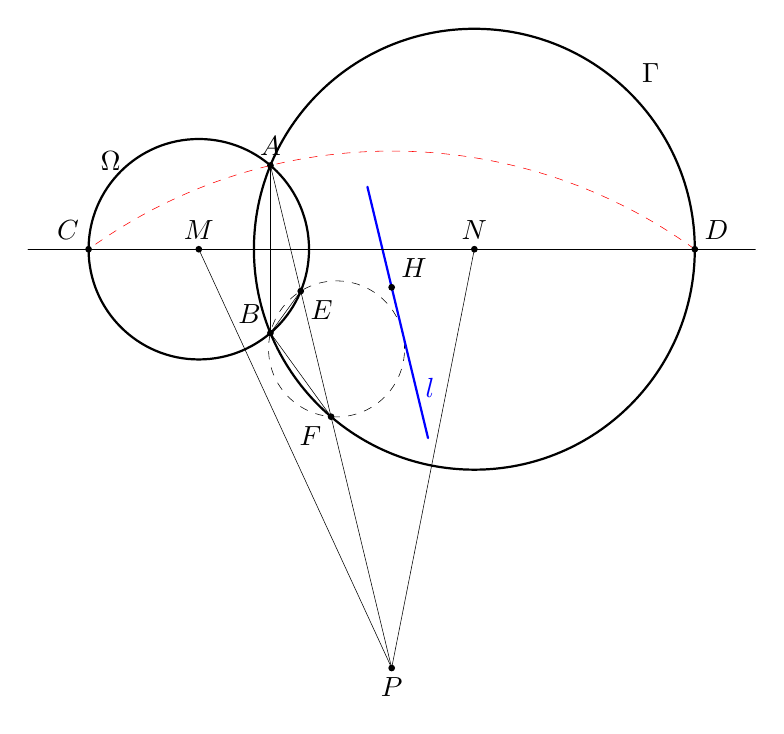
\begin{tikzpicture}[scale=0.7]
      % --- 1. 定義圓心 M, N 與半徑 ---
      \tkzDefPoint(-2,0){M}
      \tkzDefPoint(3,0){N}
      \def\rO{2}
      \def\rG{4}
      
      % --- 2. 定義直線 MN 上的 C, D (確保 C, M, N, D 順序) ---
      \tkzDefPoint(-2-\rO,0){C}
      \tkzDefPoint(3+\rG,0){D}
      
      % --- 3. 繪製兩圓 Omega, Gamma ---
      \tkzDrawCircle[thick,black](M,C)
      \tkzDrawCircle[thick,black](N,D)
      
      % --- 4. 求兩圓交點 A, B ---
      \tkzInterCC(M,C)(N,D) \tkzGetPoints{A}{B}
      
      % --- 5. 定義 P 為三角形 ACD 的外心 ---
      \tkzCircumCenter(A,C,D) \tkzGetPoint{P}
      %\tkzDrawCircle[dashed, cyan](P,A) % 繪製 ACD 的外接圓供參考
      \tkzDrawArc[color=red, dashed](P,D)(C)
      % --- 6. 構造割線 AP 並求交點 E, F ---
      \tkzInterLC(A,P)(M,C) \tkzGetPoints{E}{A_tmp}
      \tkzInterLC(A,P)(N,D) \tkzGetPoints{A_tmp2}{F}
      
      % --- 7. 計算三角形 PMN 的垂心 H ---
      \tkzOrthoCenter(P,M,N) \tkzGetPoint{H}
      
      % --- 8. 繪製三角形 BEF 的外接圓 ---
      \tkzCircumCenter(B,E,F) \tkzGetPoint{O_BEF}
      \tkzDrawCircle[dashed, black](O_BEF,B)
      
      % --- 9. 繪製通過 H 且平行於 AP 的切線 l ---
      \tkzDefLine[parallel=through H](A,P) \tkzGetPoint{l_dir}
      \tkzDrawLine[blue, thick, add=0.2 and -0.7](H,l_dir)
      
      % --- 10. 繪製線段與標籤 ---
      \tkzDrawLines[add=0.1 and 0.1](C,D)
      \tkzDrawSegments(A,P P,M P,N A,B B,E B,F)
      \tkzDrawPoints[fill=black](M,N,A,B,C,D,E,F,P,H)
      
      \tkzLabelPoints[above](M,N)
      \tkzLabelPoints[above left](C)
      \tkzLabelPoints[above right](D,H)
      \tkzLabelPoints[above left](B)
      \tkzLabelPoints[above](A)
      \tkzLabelPoints[below](P)
      \tkzLabelPoints[below right](E)
      \tkzLabelPoints[below left](F)
      
      \node at (-2-\rO*0.8,\rO*0.8) {$\Omega$};
      \node at (3+\rG*0.8,\rG*0.8) {$\Gamma$};
      \coordinate (l_1) at ($(H)!0.2!(l_dir)$);
      \node[blue, right] at (l_1) {$l$};

  \end{tikzpicture}
\end{center} 
%================ Problem 1 ================%
\newpage
%================ Solution 1 ================%
\INDEX{證明：}\INDEX{證明：}首先，目前仍未知直線$l$與$\triangle{BEF}$的外接圓是否存在交點，如果要用「證明交點為切點」的方法來證明，
必須先證明兩者之間存在交點，這個方法只會增加證明的難度。

既然如此，那麼更加不可能使用「切割線定理」來證明命題，因為切割線定理的前提是已知兩者相交。

經過篩選，目前可以使用的證明方法就有「直線$l$與$\triangle{BEF}$外接圓圓心的距離$d_1$等於此外接圓半徑$R_1$」。
\begin{center} % 子圖 1
  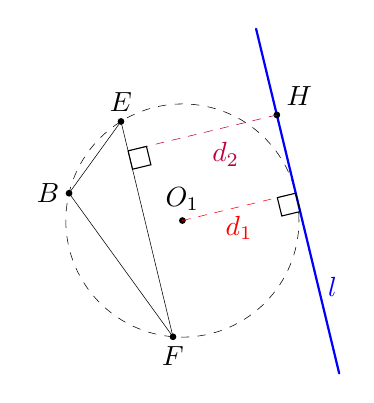
\begin{tikzpicture}[scale=1.2]
    % --- 1. 定義圓心 M, N 與半徑 ---
    \tkzDefPoint(-2,0){M}
    \tkzDefPoint(3,0){N}
    \def\rO{2}
    \def\rG{4}
    
    % --- 2. 定義直線 MN 上的 C, D (確保 C, M, N, D 順序) ---
    \tkzDefPoint(-2-\rO,0){C}
    \tkzDefPoint(3+\rG,0){D}
    
    % --- 3. 繪製兩圓 Omega, Gamma ---
    %\tkzDrawCircle[thick,black](M,C)
    %\tkzDrawCircle[thick,black](N,D)
    
    % --- 4. 求兩圓交點 A, B ---
    \tkzInterCC(M,C)(N,D) \tkzGetPoints{A}{B}
    
    % --- 5. 定義 P 為三角形 ACD 的外心 ---
    \tkzCircumCenter(A,C,D) \tkzGetPoint{P}
    %\tkzDrawCircle[dashed, cyan](P,A) % 繪製 ACD 的外接圓供參考
    %\tkzDrawArc[color=red, dashed](P,D)(C)
    % --- 6. 構造割線 AP 並求交點 E, F ---
    \tkzInterLC(A,P)(M,C) \tkzGetPoints{E}{A_tmp}
    \tkzInterLC(A,P)(N,D) \tkzGetPoints{A_tmp2}{F}
    
    % --- 7. 計算三角形 PMN 的垂心 H ---
    \tkzOrthoCenter(P,M,N) \tkzGetPoint{H}
    
    % --- 8. 繪製三角形 BEF 的外接圓 ---
    \tkzCircumCenter(B,E,F) \tkzGetPoint{O_1}
    \tkzDrawCircle[dashed, black](O_1,B)
    
    % --- 9. 繪製通過 H 且平行於 AP 的切線 l ---
    \tkzDefLine[parallel=through H](A,P) \tkzGetPoint{l_dir}
    \tkzDrawLine[blue, thick, add=0.1 and -0.7](H,l_dir)
    
    % --- 10. 繪製線段與標籤 ---
    %\tkzDrawLines[add=0.1 and 0.1](C,D)
    %\tkzDrawSegments(A,P P,M P,N A,B B,E B,F)
    %\tkzDrawPoints[fill=black](M,N,A,B,C,D,E,F,P,H)
    \tkzDrawPoints[fill=black](B,E,F,H,O_1)
    %\tkzLabelPoints[above](M,N)
    %\tkzLabelPoints[above left](C)
    %\tkzLabelPoints[above right](D,H)
    \tkzLabelPoints[above right](H)
    \tkzLabelPoints[left](B)
    %\tkzLabelPoints[above](A)
    %\tkzLabelPoints[below](P)
    \tkzLabelPoints[above](E)
    \tkzLabelPoints[below](F)
    \tkzLabelPoints[above](O_1)
    
    %\node at (-2-\rO*0.8,\rO*0.8) {$\Omega$};
    %\node at (3+\rG*0.8,\rG*0.8) {$\Gamma$};
    
    \coordinate (l_1) at ($(H)!0.2!(l_dir)$);
    \node[blue, right] at (l_1) {$l$};
    % 1. 找出 O1 在直線 (H, l_dir) 上的投影點（垂足），命名為 K
    \tkzDefPointBy[projection = onto H--l_dir](O_1) \tkzGetPoint{K}

    % 2. 繪製垂線段 O1K
    \tkzDrawSegment[color=red, dashed](O_1,K)

    % 3. 繪製直角符號
    \tkzMarkRightAngle[size=0.2](O_1,K,l_dir)

    \coordinate (d_1) at ($(O_1)!0.5!(K)$);
    \node[red, below] at (d_1) {$d_1$};
    \tkzDrawSegments(B,E B,F E,F)

     % 1. 找出 H 在直線 (E, F) 上的投影點（垂足），命名為 M
    \tkzDefPointBy[projection = onto E--F](H) \tkzGetPoint{M}

    % 2. 繪製垂線段 O1K
    \tkzDrawSegment[color=purple, dashed](H,M)

    % 3. 繪製直角符號
    \tkzMarkRightAngle[size=0.2](H,M,F)
    \coordinate (d_2) at ($(H)!0.5!(M)$);
    \node[purple, below right] at (d_2) {$d_2$};
  \end{tikzpicture}
\end{center}
現在把幾何圖的子圖放大，並記一對平行線$\left(EF,l\right)$之間的距離為$d_2$，則原命題等價於下方的命題一：
\begin{equation}
  d_1=R_1\Leftrightarrow d_2=R_1+\left\{O_1\text{到}EF\text{的距離}\right\}=R_1-R_1\cos{\angle{EBF}}
\end{equation}
同時，$d_2$ 的長度等於 $H$ 到 $EF$ 的距離。另一方面，$H$為$\triangle{BEF}$的垂心，且$P$在直線$EF$上，所以連結$HP$是必然的。
\begin{center} % 子圖 2
  \begin{tikzpicture}[rotate=75, scale=1.2]
    % --- 1. 定義圓心 M, N 與半徑 ---
    \tkzDefPoint(-2,0){M}
    \tkzDefPoint(3,0){N}
    \def\rO{2}
    \def\rG{4}
    
    % --- 2. 定義直線 MN 上的 C, D (確保 C, M, N, D 順序) ---
    \tkzDefPoint(-2-\rO,0){C}
    \tkzDefPoint(3+\rG,0){D}
    
    % --- 3. 繪製兩圓 Omega, Gamma ---
    %\tkzDrawCircle[thick,black](M,C)
    %\tkzDrawCircle[thick,black](N,D)
    
    % --- 4. 求兩圓交點 A, B ---
    \tkzInterCC(M,C)(N,D) \tkzGetPoints{A}{B}
    
    % --- 5. 定義 P 為三角形 ACD 的外心 ---
    \tkzCircumCenter(A,C,D) \tkzGetPoint{P}
    %\tkzDrawCircle[dashed, cyan](P,A) % 繪製 ACD 的外接圓供參考
    %\tkzDrawArc[color=red, dashed](P,D)(C)
    % --- 6. 構造割線 AP 並求交點 E, F ---
    \tkzInterLC(A,P)(M,C) \tkzGetPoints{E}{A_tmp}
    \tkzInterLC(A,P)(N,D) \tkzGetPoints{A_tmp2}{F}
    
    % --- 7. 計算三角形 PMN 的垂心 H ---
    \tkzOrthoCenter(P,M,N) \tkzGetPoint{H}
    
    % --- 8. 繪製三角形 BEF 的外接圓 ---
    \tkzCircumCenter(B,E,F) \tkzGetPoint{O_1}
    \tkzDrawCircle[dashed, black](O_1,B)
    
    % --- 9. 繪製通過 H 且平行於 AP 的切線 l ---
    \tkzDefLine[parallel=through H](A,P) \tkzGetPoint{l_dir}
    \tkzDrawLine[blue, thick, add=0.1 and -0.7](H,l_dir)
    
    % --- 10. 繪製線段與標籤 ---
    %\tkzDrawLines[add=0.1 and 0.1](C,D)
    %\tkzDrawSegments(A,P P,M P,N A,B B,E B,F)
    %\tkzDrawPoints[fill=black](M,N,A,B,C,D,E,F,P,H)
    \tkzDrawPoints[fill=black](B,E,F,H,P)
    %\tkzLabelPoints[above](M,N)
    %\tkzLabelPoints[above left](C)
    %\tkzLabelPoints[above right](D,H)
    \tkzLabelPoints[above](H)
    \tkzLabelPoints[below](B)
    %\tkzLabelPoints[above](A)
    \tkzLabelPoints[below](P)
    \tkzLabelPoints[left](E)
    \tkzLabelPoints[below right](F)
    %\tkzLabelPoints[above](O_1)
    
    %\node at (-2-\rO*0.8,\rO*0.8) {$\Omega$};
    %\node at (3+\rG*0.8,\rG*0.8) {$\Gamma$};
    
    \coordinate (l_1) at ($(H)!0.2!(l_dir)$);
    \node[blue, above] at (l_1) {$l$};
    % 1. 找出 O1 在直線 (H, l_dir) 上的投影點（垂足），命名為 K
    %\tkzDefPointBy[projection = onto H--l_dir](O_1) \tkzGetPoint{K}

    % 2. 繪製垂線段 O1K
    %\tkzDrawSegment[color=red, dashed](O_1,K)

    % 3. 繪製直角符號
    %\tkzMarkRightAngle[size=0.2](O_1,K,l_dir)

    %\coordinate (d_1) at ($(O_1)!0.5!(K)$);
    %\node[red, below] at (d_1) {$d_1$};
    \tkzDrawSegments(B,E B,F E,P)
    \tkzDrawSegments[dashed](H,P)

     % 1. 找出 H 在直線 (E, F) 上的投影點（垂足），命名為 M
    \tkzDefPointBy[projection = onto E--F](H) \tkzGetPoint{M}

    % 2. 繪製垂線段 O1K
    \tkzDrawSegment[color=purple, dashed](H,M)

    % 3. 繪製直角符號
    \tkzMarkRightAngle[size=0.2](H,M,F)
    \coordinate (d_2) at ($(H)!0.5!(M)$);
    \node[purple, below right] at (d_2) {$d_2$};

\end{tikzpicture}
\end{center}
所以命題一等價於下方的命題二：
\begin{equation}
  HP\sin{\angle{HPE}}=d_2=R_1\left(1-\cos{\angle{EBF}}\right)
\end{equation}
現在只剩下$R_1$仍未計算出來，所以下一步就是計算$R_1$的長度。對$\triangle{BEF}$使用正弦定理可得：
\begin{equation}
  2R_1=\frac{BE}{\sin{\angle{BFE}}}\left(=\frac{BF}{\sin{\angle{BEF}}}\right)
\end{equation}
所以命題二等價於下方的命題三：
\begin{equation}
  HP\sin{\angle{HPE}}=\frac{BE}{2\sin{\angle{BFE}}}\left(1-\cos{\angle{EBF}}\right)
\end{equation}

下一步，我們需要把命題三中的各個量轉化成與$E,F$無關的量：
\begin{itemize}
  \item 因為$A,B$是圓$\Omega$與$\Gamma$的交點，所以$AB$是兩圓的公共弦，因此$AB\perp MN$。
  同時，$H$是$\triangle{PMN}$的垂心，所以$PH\perp MN$。由此可得 $AB\parallel PH$，所以$$\angle{HPE}=\angle{BAP}$$
  \item 記圓$\Omega$的半徑為$R_M$，對圓$\Omega$使用正弦定理：$$BE=2R_M\sin{\angle{BAE}}=2R_M\sin{\angle{BAP}}$$
  \item 在圓$\Gamma$中使用Angle Chasing：$\angle{BFE}=\angle{BFA}=\angle{BDA}$。記圓$\Gamma$的半徑為$R_N$，對圓$\Gamma$使用正弦定理：
  $$\sin{\angle{BFE}}=\sin{\angle{BDA}}=\frac{BA}{2R_N}$$
  \item $$\angle{EBF}=180^{\circ}-\angle{BEF}-\angle{BFE}=180^{\circ}-\angle{BEF}-\angle{BDA}$$
  在圓$\Gamma$中使用Angle Chasing：$$\angle{BEF}=\angle{BCA}$$
  所以有$$\angle{EBF}=180^{\circ}-\angle{BCA}-\angle{BDA}$$
  \iffalse
  利用圓周角定理可知
  $$\begin{cases}\angle{BCA}=\frac{1}{2}\angle{BMA}=\angle{AMN}\\ \angle{BDA}=\frac{1}{2}\angle{BNA}=\angle{ANM}\end{cases}$$
  因此
  $$\angle{EBF}=180^{\circ}-\angle{AMN}-\angle{ANM}=\angle{MAN}$$
  \fi
\end{itemize}
將上述結果代入命題三，可得命題四：
\begin{align}
  HP\sin{\angle{BAP}}&=\frac{2R_M\sin{\angle{BAP}}}{2\cdot\frac{BA}{2R_N}}
  \left[1-\cos{\left(180^{\circ}-\angle{BCA}-\angle{BDA}\right)}\right]\notag\\
  &=\frac{2R_MR_N\sin{\angle{BAP}}}{AB}\left[1+\cos{\left(\angle{BCA}+\angle{BDA}\right)}\right]
\end{align}
命題四兩邊都存在$\sin{\angle{BAP}}$，所以可以約去，得到命題五：
\begin{equation}
  HP=\frac{2R_MR_N}{AB}\left[1+\cos{\left(\angle{BCA}+\angle{BDA}\right)}\right]
\end{equation}
下一步，我們需要想辦法把$HP$的長度表示成與$H$無關的量，所以我把另一個幾何圖的子圖放大
\begin{center} % 子圖 3
  \begin{tikzpicture}[rotate=-90, scale=0.6]
    \tkzDefPoint(-2,0){M}
    \tkzDefPoint(3,0){N}
    \def\rO{2}
    \def\rG{4}
    \tkzDefPoint(-2-\rO,0){C}
    \tkzDefPoint(3+\rG,0){D}
    \tkzInterCC(M,C)(N,D) \tkzGetPoints{A}{B}
    \tkzCircumCenter(A,C,D) \tkzGetPoint{P}
    \tkzInterLC(A,P)(M,C) \tkzGetPoints{E}{A_tmp}
    \tkzInterLC(A,P)(N,D) \tkzGetPoints{A_tmp2}{F}
    \tkzOrthoCenter(P,M,N) \tkzGetPoint{H}
    \tkzDrawSegments(M,N P,N P,M)
    \tkzDrawPoints[fill=black](M,N,P,H)    
    \tkzLabelPoints[right](M,N)
    \tkzLabelPoints[above left](H)
    \tkzLabelPoints[below](P)
  \end{tikzpicture}
\end{center}
如果大家還記得「垂心-重心-外心」關係的話，很快就能得到：
$$
\overrightarrow{O_2H}=\overrightarrow{O_2P}+\overrightarrow{O_2M}+\overrightarrow{O_2N}
\Leftrightarrow\overrightarrow{PH}=\overrightarrow{O_2M}+\overrightarrow{O_2N}
$$
其中$O_2$為$\triangle{PMN}$的外心，為了讀者能更清晰地去計算，下圖為添加了$O_2$的幾何圖子圖：
\begin{center} % 子圖 4
  \begin{tikzpicture}[rotate=-90, scale=0.6]
    \tkzDefPoint(-2,0){M}
    \tkzDefPoint(3,0){N}
    \def\rO{2}
    \def\rG{4}
    \tkzDefPoint(-2-\rO,0){C}
    \tkzDefPoint(3+\rG,0){D}
    \tkzInterCC(M,C)(N,D) \tkzGetPoints{A}{B}
    \tkzCircumCenter(A,C,D) \tkzGetPoint{P}
    \tkzInterLC(A,P)(M,C) \tkzGetPoints{E}{A_tmp}
    \tkzInterLC(A,P)(N,D) \tkzGetPoints{A_tmp2}{F}
    \tkzOrthoCenter(P,M,N) \tkzGetPoint{H}
    \tkzCircumCenter(P,M,N) \tkzGetPoint{O_2}
    \tkzDrawCircle[dashed, black](O_2,M)
    \tkzDrawSegments(M,N P,N P,M)
    \tkzDrawSegments[dashed, black](O_2,M O_2,N)
    \tkzDrawPoints[fill=black](M,N,P,H,O_2)   
    \tkzLabelPoints[right](M,N)
    \tkzLabelPoints[above left](H)
    \tkzLabelPoints[below](P)
    \tkzLabelPoints[below](O_2)
  \end{tikzpicture}
\end{center}
記此外接圓半徑為$R_2$，由幾何關係可以算得
\begin{align*}
  HP&=\left|\overrightarrow{O_2M}+\overrightarrow{O_2N}\right|=2R_2\cos{\frac{\angle{MO_2N}}{2}}\\
  &=2R_2\cos{\angle{MPN}}=\frac{MN}{\sin{}\angle{MPN}}\cos{\angle{MPN}}\\
  &=MN\cot{\angle{MPN}}
\end{align*}
代入命題五可得
\begin{equation}
  MN\cot{\angle{MPN}}=\frac{2R_MR_N}{AB}\left[1+\cos{\left(\angle{BCA}+\angle{BDA}\right)}\right]
\end{equation}
現在整理當前的幾何圖
\begin{center} % 子圖 5
  \begin{tikzpicture}[scale=0.8]
    \tkzDefPoint(-2,0){M}
    \tkzDefPoint(3,0){N}
    \def\rO{2}
    \def\rG{4} 
    \tkzDefPoint(-2-\rO,0){C}
    \tkzDefPoint(3+\rG,0){D}
    \tkzDrawCircle[thick,black](M,C)
    \tkzDrawCircle[thick,black](N,D)
    \tkzInterCC(M,C)(N,D) \tkzGetPoints{A}{B}
    \tkzCircumCenter(A,C,D) \tkzGetPoint{P}
    \tkzDrawArc[color=red, dashed](P,D)(C)
    \tkzDrawLines[add=0.1 and 0.1](C,D)
    \tkzDrawSegments(A,P P,M P,N A,B)
    \tkzDrawPoints[fill=black](M,N,A,B,C,D,P)
    \tkzLabelPoints[above](M,N)
    \tkzLabelPoints[above left](C)
    \tkzLabelPoints[above right](D)
    \tkzLabelPoints[above left](B)
    \tkzLabelPoints[above](A)
    \tkzLabelPoints[below](P)
    \node at (-2-\rO*0.8,\rO*0.8) {$\Omega$};
    \node at (3+\rG*0.8,\rG*0.8) {$\Gamma$};
  \end{tikzpicture}
\end{center}
下一步，我們需要把$\angle{MPN}$表示成與$P$無關的量，即把$P$點消去：

因為$P$為$\triangle{ACD}$的外心，而$M$為$\triangle{ACB}$的外心，所以直線$MP$為$AC$的中垂線。
同理，直線$NP$為$AD$的中垂線。

為了能夠更清楚地解釋，筆者再提取了幾何圖的子圖：
\begin{center} % 子圖 6
  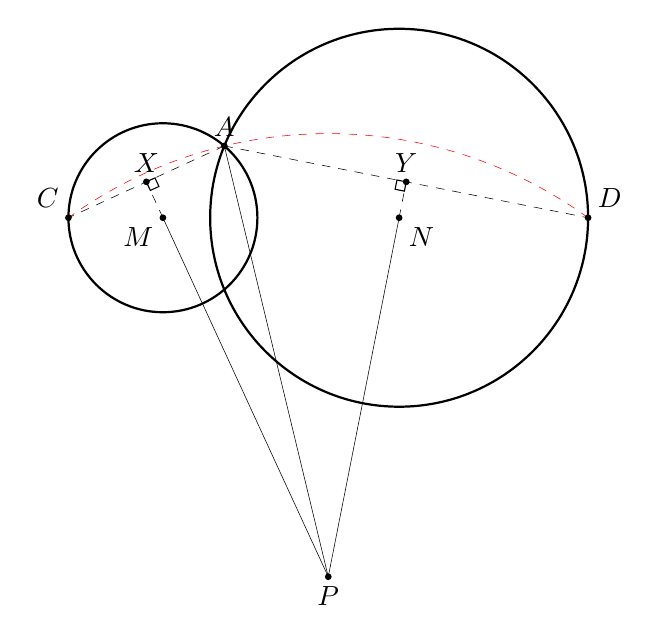
\begin{tikzpicture}[scale=0.6]
    \tkzDefPoint(-2,0){M}
    \tkzDefPoint(3,0){N}
    \def\rO{2}
    \def\rG{4}
    \tkzDefPoint(-2-\rO,0){C}
    \tkzDefPoint(3+\rG,0){D}
    \tkzDrawCircle[thick,black](M,C)
    \tkzDrawCircle[thick,black](N,D)
    \tkzInterCC(M,C)(N,D) \tkzGetPoints{A}{B}
    \tkzCircumCenter(A,C,D) \tkzGetPoint{P}
    \tkzDrawArc[color=red, dashed](P,D)(C)
    \tkzInterLL(M,P)(A,C) \tkzGetPoint{X}
    \tkzInterLL(N,P)(A,D) \tkzGetPoint{Y}
    \tkzDrawSegments(A,P P,M P,N)
    \tkzDrawSegments[dashed](M,X A,C N,Y A,D)
    \tkzDrawPoints[fill=black](M,N,A,C,D,P,X,Y)
    \tkzLabelPoints[below left](M)
    \tkzLabelPoints[below right](N)
    \tkzLabelPoints[above left](C)
    \tkzLabelPoints[above right](D)
    \tkzLabelPoints[above](A)
    \tkzLabelPoints[below](P)
    \tkzLabelPoints[above](X,Y)
    \tkzMarkRightAngle[size=0.2](M,X,A)
    \tkzMarkRightAngle[size=0.2](N,Y,A)
  \end{tikzpicture}
\end{center}
記$PM$交$AC$於$X$，$PN$交$AD$於$Y$，由$PM\perp AC$和$PN\perp AD$可知$A,X,P,Y$四點共圖，所以
$$\angle{MPN}=\angle{XPY}=180^{\circ}-\angle{XAY}=180^{\circ}-\angle{CAD}$$
代入至命題五可得：
\begin{equation}
  \frac{2R_MR_N}{AB}\left[1+\cos{\left(\angle{BCA}+\angle{BDA}\right)}\right]
  =MN\cot{\left(180^{\circ}-\angle{CAD}\right)}=-MN\cot{\angle{CAD}}
\end{equation}
現在整理當前的幾何圖
\begin{center} % 子圖 7
  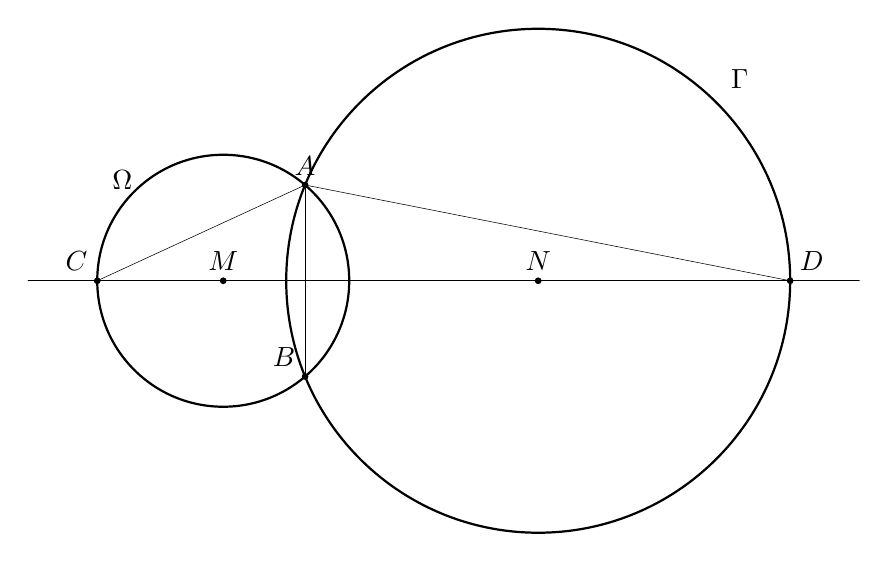
\begin{tikzpicture}[scale=0.8]
    \tkzDefPoint(-2,0){M}
    \tkzDefPoint(3,0){N}
    \def\rO{2}
    \def\rG{4}
    \tkzDefPoint(-2-\rO,0){C}
    \tkzDefPoint(3+\rG,0){D}
    \tkzDrawCircle[thick,black](M,C)
    \tkzDrawCircle[thick,black](N,D)
    \tkzInterCC(M,C)(N,D) \tkzGetPoints{A}{B}
    \tkzDrawLines[add=0.1 and 0.1](C,D)
    \tkzDrawSegments(A,B C,A A,D)
    \tkzDrawPoints[fill=black](M,N,A,B,C,D)
    \tkzLabelPoints[above](M,N)
    \tkzLabelPoints[above left](C)
    \tkzLabelPoints[above right](D)
    \tkzLabelPoints[above left](B)
    \tkzLabelPoints[above](A)
    \node at (-2-\rO*0.8,\rO*0.8) {$\Omega$};
    \node at (3+\rG*0.8,\rG*0.8) {$\Gamma$};
  \end{tikzpicture}
\end{center}
下一步，我們要消去$C,D$兩點：
利用圓周角定理可知
$$
\begin{cases}
  \angle{BCA}=\frac{1}{2}\angle{BMA}=\angle{AMN}\\ 
  \angle{BDA}=\frac{1}{2}\angle{BNA}=\angle{ANM}
\end{cases}
$$
所以有
$$
\angle{BCA}+\angle{BDA}=\angle{AMN}+\angle{ANM}=180^{\circ}-\angle{MAN}
$$
另一方面
\begin{align*}
  \angle{CAD}&=\angle{MAN}+\angle{CAM}+\angle{DAN}\\
  &=\angle{MAN}+\angle{MAC}+\angle{NDA}\\
  &=\angle{MAN}+\frac{1}{2}\left(\angle{BCA}+\angle{BDA}\right)\\
  &=\angle{MAN}+\frac{1}{2}\left(180^{\circ}-\angle{MAN}\right)\\
  &=90^{\circ}+\frac{1}{2}\angle{MAN}
\end{align*}
因此命題五等價於下方的命題六：
\begin{align}
  &\frac{2R_MR_N}{AB}\left[1+\cos{\left(180^{\circ}-\angle{MAN}\right)}\right]
  =-MN\cot{\left(90^{\circ}+\frac{1}{2}\angle{MAN}\right)}\notag\\
  \Leftrightarrow\quad&\frac{2R_MR_N}{AB}\left(1-\cos{\angle{MAN}}\right)
  =MN\tan{\frac{\angle{MAN}}{2}}\notag\\
  \Leftrightarrow\quad&\frac{2R_MR_N}{AB}\cdot2\sin^2{\frac{\angle{MAN}}{2}}=MN\cdot\tan{\frac{\angle{MAN}}{2}}\notag\\
  \Leftrightarrow\quad&\frac{2R_MR_N}{AB}\cdot2\sin{\frac{\angle{MAN}}{2}}\cos{\frac{\angle{MAN}}{2}}=MN\notag\\
  \Leftrightarrow\quad&\frac{2R_MR_N}{AB}\sin{\angle{MAN}}=MN\notag\\
  \Leftrightarrow\quad&2R_MR_N\sin{\angle{MAN}}=MN\cdot AB
\end{align}
現在整理當前的幾何圖
\begin{center} % 子圖 8
  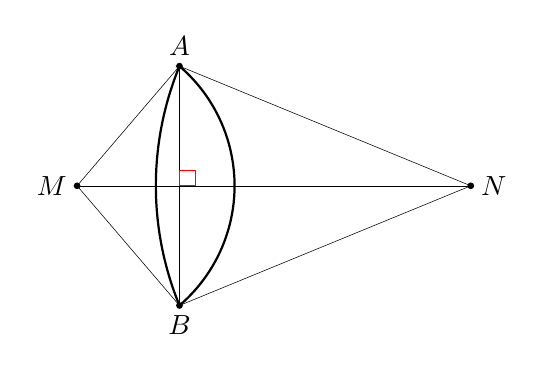
\begin{tikzpicture}[scale=1]
    \tkzDefPoint(-2,0){M}
    \tkzDefPoint(3,0){N}
    \def\rO{2}
    \def\rG{4}
    \tkzDefPoint(-2-\rO,0){C}
    \tkzDefPoint(3+\rG,0){D}
    \tkzInterCC(M,C)(N,D) \tkzGetPoints{A}{B}
    \tkzDrawArc[thick,black](M,B)(A)
    \tkzDrawArc[thick,black](N,A)(B)
    \tkzDrawSegments(A,B A,M A,N B,M B,N M,N)
    \tkzDrawPoints[fill=black](M,N,A,B)
    \tkzLabelPoints[left](M)
    \tkzLabelPoints[right](N)
    \tkzLabelPoints[below](B)
    \tkzLabelPoints[above](A)
    \tkzInterLL(M,N)(A,B) \tkzGetPoint{K}
    \tkzMarkRightAngle[size=0.2, red](A,K,N)
  \end{tikzpicture}
\end{center}
因為 $MN\perp AB$，所以
\begin{equation}
  \left[AMBN\right]=\frac{1}{2}MN\cdot AB\label{eq:Area_AMBN_1}
\end{equation}
另一方面，易知 $\triangle{AMN}\cong\triangle{BMN}$，所以
\begin{align}
  \left[AMBN\right]&=\left[\triangle{AMN}\right]+\left[\triangle{BMN}\right]\notag\\
  &=2\left[\triangle{AMN}\right]\notag\\
  &=AM\cdot AN\sin{\angle{MAN}}\notag\\
  &=R_MR_N\sin{\angle{MAN}}\label{eq:Area_AMBN_2}
\end{align}
聯立式\eqref{eq:Area_AMBN_1}與式\eqref{eq:Area_AMBN_2}可得
\begin{align}
  &\frac{1}{2}MN\cdot AB=R_MR_N\sin{\angle{MAN}}\notag\\
  \Leftrightarrow\quad&2R_MR_N\sin{\angle{MAN}}=MN\cdot AB
\end{align}
由此可證得命題六成立，即原命題成立。
%================ Solution 1 ================%
\newpage
%================ Problem 2 ================%
\INDEX{問題2}設四邊形$ABCD$是梯形，$AB\parallel CD$且$AB<CD$。
直線$AD$和$BC$交於點$P$。$\triangle{ABC}$上的一點$X\neq C$滿足$PX=PC$，
$\triangle{ABD}$上的一點$Y\neq D$滿足$PY=PD$直線$AX$與$BY$交於點$Q$。

\textbf{求證：}$PQ\parallel AB$
\begin{center} % p2 示意圖
  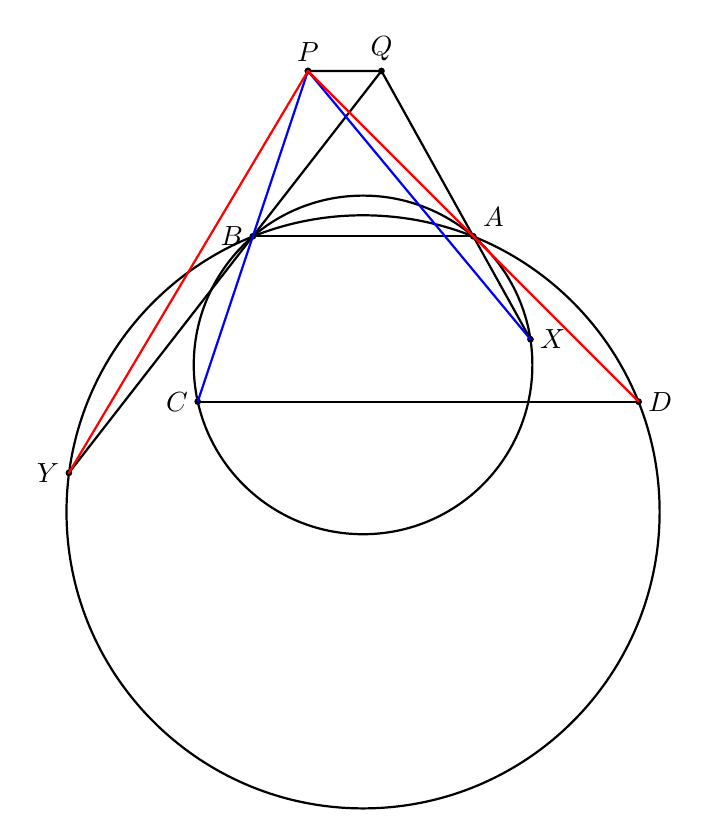
\begin{tikzpicture}[scale=0.7]
    \tkzDefPoint(2,3){A}
    \tkzDefPoint(-2,3){B}
    \tkzDefPoint(-3,0){C}
    \tkzDefPoint(5,0){D}
    \tkzInterLL(A,D)(B,C) \tkzGetPoint{P}
    \tkzCircumCenter(A,B,C) \tkzGetPoint{O_1}
    \tkzCircumCenter(A,B,D) \tkzGetPoint{O_2}
    \tkzInterCC(O_1,C)(P,C) \tkzGetPoints{C_tmp}{X}
    \tkzInterCC(O_2,D)(P,D) \tkzGetPoints{Y}{D_tmp}
    \tkzDrawCircle[black,thick](O_1,A)
    \tkzDrawCircle[black,thick](O_2,A)
    \tkzInterLL(A,X)(B,Y) \tkzGetPoint{Q}
    \tkzDrawPoints[fill=black](A,B,C,D,P,X,Y,P,Q)
    \tkzLabelPoints[right](D)
    \tkzLabelPoints[above right](A)
    \tkzLabelPoints[left](B,C)
    \tkzLabelPoints[above](P)
    \tkzLabelPoints[above](Q)
    \tkzLabelPoints[right](X)
    \tkzLabelPoints[left](Y)
    \tkzDrawSegments[black, thick](A,B C,D P,Q X,Q Y,Q)
    \tkzDrawSegments[blue, thick](P,X P,C)
    \tkzDrawSegments[red, thick](P,Y P,D)
  \end{tikzpicture}
\end{center}
%================ Problem 2 ================%
\newpage
%================ Solution 2 ================%
\INDEX{證明：}\setcounter{equation}{0}
要證明兩直線平行，方法不外乎以下幾種：
\begin{enumerate}[label=(\roman*)]
  \item 找到相等的同位角、內錯角
  \item 找到互補的同旁內角
  \item 向量平行
  \item 找到兩點（兩個點同一在直線上或分別在兩條直線都可）到另一條直線的距離相等
\end{enumerate}
如果要用第(i)種或第(ii)種方法，
那麼至少要研究 $\angle{PQA}$、$\angle{PQB}$、
$\angle{QPA}$和$\angle{QPB}$ 之間的其中一個角。
因為這些角都直接涉及到直線$PQ$，所以很難去轉換這些角。

要用第(iii)種方法，其困難在於寫出交點向量。
非常不幸地，本題中含有大量交點，而且是圓與圓的交點，所以此方法亦不適用。

要用第(iv)種方法，
可以嘗試以「$P$到$AB$的距離$d_{P,AB}$等於$Q$到$AB$的距離$d_{Q,AB}$」作為切入點。
同時，因為$AB\parallel CD$，所以若原命題得證，則必定有「$P$到$CD$的距離$d_{P,CD}$等於$Q$到$AB$的距離$d_{Q,CD}$」成立。

一般如果題目已知存在一對平行線，則最好把要論證的「數值」由「角度、長度、面積」變成「比值」，因為這樣可以配合相似三角形得到更多幾何關係。
\begin{center} % 子圖 1
  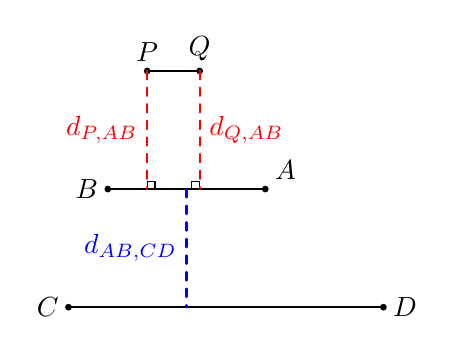
\begin{tikzpicture}[scale=0.5]
    \tkzDefPoint(2,3){A}
    \tkzDefPoint(-2,3){B}
    \tkzDefPoint(-3,0){C}
    \tkzDefPoint(5,0){D}
    \tkzInterLL(A,D)(B,C) \tkzGetPoint{P}
    \tkzCircumCenter(A,B,C) \tkzGetPoint{O_1}
    \tkzCircumCenter(A,B,D) \tkzGetPoint{O_2}
    \tkzInterCC(O_1,C)(P,C) \tkzGetPoints{C_tmp}{X}
    \tkzInterCC(O_2,D)(P,D) \tkzGetPoints{Y}{D_tmp}
    \tkzInterLL(A,X)(B,Y) \tkzGetPoint{Q}
    \tkzDrawPoints[fill=black](A,B,C,D,P,Q)
    \tkzLabelPoints[right](D)
    \tkzLabelPoints[above right](A)
    \tkzLabelPoints[left](B,C)
    \tkzLabelPoints[above](P)
    \tkzLabelPoints[above](Q)
    \tkzDrawSegments[black, thick](A,B C,D P,Q)
    \tkzDefPointBy[projection = onto B--A](P) \tkzGetPoint{P_1}
    \tkzDefPointBy[projection = onto B--A](Q) \tkzGetPoint{Q_1}
    \tkzDrawSegment[color=red, dashed](P,P_1)
    \tkzDrawSegment[color=red, dashed](Q,Q_1)
    \tkzMarkRightAngle[size=0.2](P,P_1,A)
    \tkzMarkRightAngle[size=0.2](Q,Q_1,B)\coordinate (d_ABCD_1) at ($(B)!0.5!(A)$);
    \tkzDefPointBy[projection = onto C--D](d_ABCD_1) \tkzGetPoint{d_ABCD_2}
    \tkzDrawSegment[color=blue, dashed, thick](d_ABCD_1,d_ABCD_2)
    \tkzDrawSegment[color=red, dashed, thick](P,P_1)
    \tkzDrawSegment[color=red, dashed, thick](Q,Q_1)
    \node[blue, left] at ($(d_ABCD_1)!0.5!(d_ABCD_2)$) {$d_{AB,CD}$};
    \node[red, left] at ($(P)!0.5!(P_1)$) {$d_{P,AB}$};
    \node[red, right] at ($(Q)!0.5!(Q_1)$) {$d_{Q,AB}$};
  \end{tikzpicture}
\end{center}

提取出原幾何圖的子圖。顯然，當原命題成立時，「$d_{P,AB}:d_{P,CD}=d_{Q,AB}:d_{Q,CD}$」也必定成立。

注意，題中的一對平行線$AB$和$CD$之間的距離$d_{AB,CD}$是一個「定值」。經過以下的等價變換
\begin{align*}
  d_{P,AB}:d_{P,CD}=d_{Q,AB}:d_{Q,CD}\Leftrightarrow\quad& \frac{d_{P,CD}}{d_{P,AB}}=\frac{d_{Q,CD}}{d_{Q,AB}}\\ 
  \Leftrightarrow\quad& \frac{d_{P,CD}}{d_{P,AB}}-1=\frac{d_{Q,CD}}{d_{Q,AB}}-1\\ 
  \Leftrightarrow\quad& \frac{d_{AB,CD}}{d_{P,AB}}=\frac{d_{AB,CD}}{d_{Q,AB}}\\ 
  \Leftrightarrow\quad& d_{P,AB}=d_{Q,AB}\Rightarrow\quad PQ\parallel AB
\end{align*}

所以原命題等價於以下的命題一：
\begin{equation}
  PQ\parallel AB\Leftrightarrow\frac{d_{P,AB}}{d_{P,CD}}=\frac{d_{Q,AB}}{d_{Q,CD}}\label{eq:p2_s1}
\end{equation}

\begin{center} % 子圖 2
  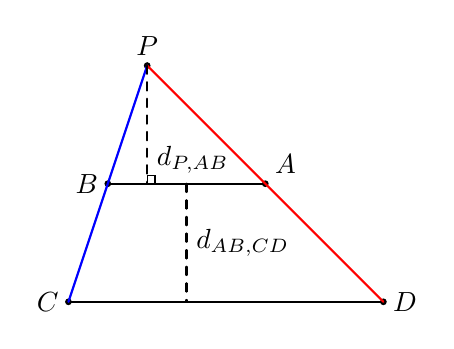
\begin{tikzpicture}[scale=0.5]
    \tkzDefPoint(2,3){A}
    \tkzDefPoint(-2,3){B}
    \tkzDefPoint(-3,0){C}
    \tkzDefPoint(5,0){D}
    \tkzInterLL(A,D)(B,C) \tkzGetPoint{P}\tkzDrawPoints[fill=black](A,B,C,D,P)
    \tkzLabelPoints[right](D)
    \tkzLabelPoints[above right](A)
    \tkzLabelPoints[left](B,C)
    \tkzLabelPoints[above](P)
    \tkzDrawSegments[black, thick](A,B C,D)
    \tkzDrawSegments[blue, thick](P,C)
    \tkzDrawSegments[red, thick](P,D)
    \tkzDefPointBy[projection = onto B--A](P) \tkzGetPoint{P_1}
    \tkzDrawSegment[color=red, dashed](P,P_1)
    \tkzMarkRightAngle[size=0.2](P,P_1,A)
    \coordinate (d_ABCD_1) at ($(B)!0.5!(A)$);
    \tkzDefPointBy[projection = onto C--D](d_ABCD_1) \tkzGetPoint{d_ABCD_2}
    \tkzDrawSegment[color=black, dashed, thick](d_ABCD_1,d_ABCD_2)
    \tkzDrawSegment[color=black, dashed, thick](P,P_1)
    \node[black, right] at ($(d_ABCD_1)!0.5!(d_ABCD_2)$) {$d_{AB,CD}$};
    \node[black, right] at ($(P)!0.8!(P_1)$) {$d_{P,AB}$};
  \end{tikzpicture}
\end{center}

第一步，研究 $d_{P,AB}:d_{P,CD}$：

因為$AB\parallel CD$，所以$\triangle{PBA}$和$\triangle{PCD}$是位似三角形，即有
\begin{equation}
  \frac{d_{P,AB}}{d_{P,CD}}=\frac{PA}{PD}=\frac{PB}{PC}=\frac{BA}{CD}\label{eq:p2_s1-1}
\end{equation}
(\ref{eq:p2_s1-1})式中我們選擇$BA/CD$的值，因為此表達式上只存在$A,B,C,D$四點，是「最簡形式」。所以命題一等價於以下的命題二：
\begin{equation}
  \frac{d_{Q,AB}}{d_{Q,CD}}=\frac{BA}{CD}\label{eq:p2_s2}
\end{equation}
留意到(\ref{eq:p2_s2})式中包含 $A,B,C,D,Q$ 五點。在原幾何圖中，已知線段已經連成了$\triangle{QAB}$，而命題二又與$CD$有關，所以我們需要令射線$QB$和$QA$與直線$CD$產生聯繫才可。

第二步，研究 $d_{Q,AB}:d_{Q,CD}$：
\begin{center} % 子圖 3
  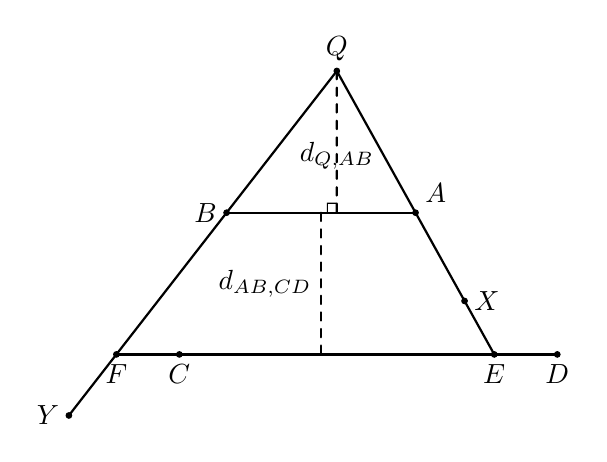
\begin{tikzpicture}[scale=0.6]
    \tkzDefPoint(2,3){A}
    \tkzDefPoint(-2,3){B}
    \tkzDefPoint(-3,0){C}
    \tkzDefPoint(5,0){D}
    \tkzInterLL(A,D)(B,C) \tkzGetPoint{P}
    \tkzCircumCenter(A,B,C) \tkzGetPoint{O_1}
    \tkzCircumCenter(A,B,D) \tkzGetPoint{O_2}
    \tkzInterCC(O_1,C)(P,C) \tkzGetPoints{C_tmp}{X}
    \tkzInterCC(O_2,D)(P,D) \tkzGetPoints{Y}{D_tmp}
    \tkzInterLL(A,X)(B,Y) \tkzGetPoint{Q}
    \tkzInterLL(A,X)(C,D) \tkzGetPoint{E}
    \tkzInterLL(B,Y)(C,D) \tkzGetPoint{F}
    \tkzDrawPoints[fill=black](A,B,C,D,E,F,Q,X,Y)
    \tkzLabelPoints[above right](A)
    \tkzLabelPoints[left](B)
    \tkzLabelPoints[below](E,F,C,D)
    \tkzLabelPoints[above](Q)
    \tkzLabelPoints[right](X)
    \tkzLabelPoints[left](Y)
    \tkzDrawSegments[black, thick](A,B F,D Q,E Q,Y)
    \tkzDefPointBy[projection = onto B--A](Q) \tkzGetPoint{Q_1}
    \tkzDrawSegment[color=red, dashed](Q,Q_1)
    \tkzMarkRightAngle[size=0.2](Q,Q_1,B)
    \coordinate (d_ABCD_1) at ($(B)!0.5!(A)$);
    \tkzDefPointBy[projection = onto C--D](d_ABCD_1) \tkzGetPoint{d_ABCD_2}
    \tkzDrawSegment[color=black, dashed, thick](d_ABCD_1,d_ABCD_2)
    \tkzDrawSegment[color=black, dashed, thick](Q,Q_1)
    \node[black, left] at ($(d_ABCD_1)!0.5!(d_ABCD_2)$) {$d_{AB,CD}$};
    \node[black] at ($(Q)!0.6!(Q_1)$) {$d_{Q,AB}$};
  \end{tikzpicture}
\end{center}
作直線$AX$與直線$CD$的交點為$E$，直線$BY$與直線$CD$的交點為$F$。\textcolor{gray}{（溫馨提示：雖然直線$AX$和直線$QA$是同一條，但是為了可以逐步消去$Q$點，在解答過程中亦盡量減少出現不出現的$Q$點；直線$BY$同理）}
因為$AB\parallel CD$，即$AB\parallel EF$，所以$\triangle{QBA}$和$\triangle{QFE}$也是位似三角形，即有
\begin{equation}
  \frac{d_{Q,AB}}{d_{Q,CD}}=\frac{QA}{QE}=\frac{QB}{QF}=\frac{BA}{FE}\label{eq:p2_s2-1}
\end{equation}
與第一步的情況一樣，我們選擇$BA/FE$的值，所以命題二等價於以下的命題三：
\begin{equation}
  \frac{BA}{FE}=\frac{BA}{CD}\Leftrightarrow FE=CD\Leftrightarrow FC=ED\label{eq:p2_s3}
\end{equation}
至此，我們成功消去$Q$點，整理當前的幾何圖：
\begin{center} % 子圖 4
  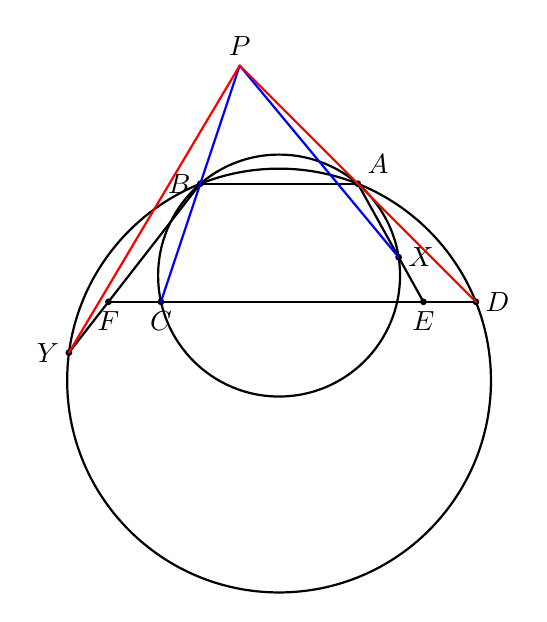
\begin{tikzpicture}[scale=0.5]
    \tkzDefPoint(2,3){A}
    \tkzDefPoint(-2,3){B}
    \tkzDefPoint(-3,0){C}
    \tkzDefPoint(5,0){D}
    \tkzInterLL(A,D)(B,C) \tkzGetPoint{P}
    \tkzCircumCenter(A,B,C) \tkzGetPoint{O_1}
    \tkzCircumCenter(A,B,D) \tkzGetPoint{O_2}
    \tkzInterCC(O_1,C)(P,C) \tkzGetPoints{C_tmp}{X}
    \tkzInterCC(O_2,D)(P,D) \tkzGetPoints{Y}{D_tmp}
    \tkzDrawCircle[black,thick](O_1,A)
    \tkzDrawCircle[black,thick](O_2,A)
    \tkzInterLL(A,X)(C,D) \tkzGetPoint{E}
    \tkzInterLL(B,Y)(C,D) \tkzGetPoint{F}
    \tkzDrawPoints[fill=black](A,B,C,D,E,F,X,Y)
    \tkzLabelPoints[above right](A)
    \tkzLabelPoints[left](B)
    \tkzLabelPoints[below](E,F,C)
    \tkzLabelPoints[above](P)
    \tkzLabelPoints[right](X,D)
    \tkzLabelPoints[left](Y)
    \tkzDrawSegments[black, thick](A,B F,D A,E B,Y)
    \tkzDrawSegments[blue, thick](P,X P,C)
    \tkzDrawSegments[red, thick](P,Y P,D)
  \end{tikzpicture}
\end{center}

第三步，歸類思維：

(\ref{eq:p2_s3})式中的線段$FC$和$ED$沒有公共端點，無法簡單地形成比值關係，所以需要把目光投向「其他上層點」。

注意到，$E$點是直線$AX$與$CD$相交而得，撇除初始點$A,C,D$後，會發現$E$點是受$X$點影響的。
$X$點是由$C$點經過一些對稱變換而生成，且在$\triangle{ABC}$上，所以在腦海中可以生成一個「C類」，C類包含$\triangle{ABC}$、$\triangle{ABC}$的外接圓、$X$、$E$。

同理，另一個就是「D類」，D類包含$\triangle{ABD}$、$\triangle{ABD}$的外接圓、$Y$、$F$。

現在命題三中的兩線段$FC$和$ED$，明顯使兩個種類產生了糾纏，使得解題難度增高。我們需要做的，就是把兩個種類的糾纏部分拆開。
\begin{center} % 子圖 5
  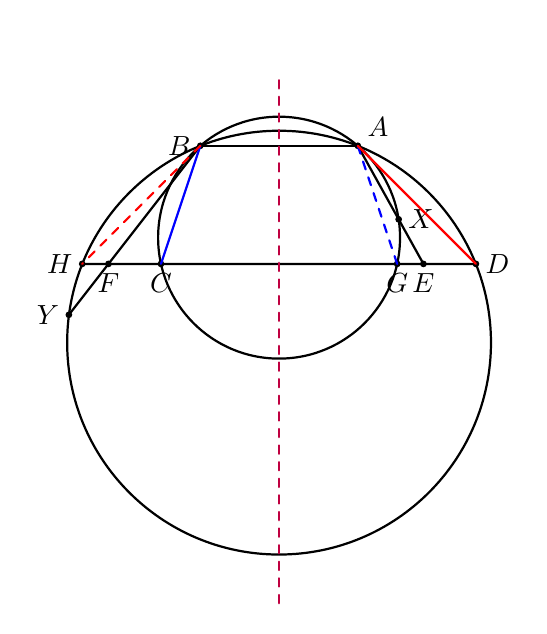
\begin{tikzpicture}[scale=0.5]
    \tkzDefPoint(2,3){A}
    \tkzDefPoint(-2,3){B}
    \tkzDefPoint(-3,0){C}
    \tkzDefPoint(5,0){D}
    \tkzInterLL(A,D)(B,C) \tkzGetPoint{P}
    \tkzCircumCenter(A,B,C) \tkzGetPoint{O_1}
    \tkzCircumCenter(A,B,D) \tkzGetPoint{O_2}
    \tkzInterCC(O_1,C)(P,C) \tkzGetPoints{C_tmp}{X}
    \tkzInterCC(O_2,D)(P,D) \tkzGetPoints{Y}{D_tmp}
    \tkzDrawCircle[black,thick](O_1,A)
    \tkzDrawCircle[black,thick](O_2,A)
    \tkzInterLL(A,X)(C,D) \tkzGetPoint{E}
    \tkzInterLL(B,Y)(C,D) \tkzGetPoint{F}
    \tkzInterLC(C,D)(O_1,A) \tkzGetPoints{C_tmp}{G}
    \tkzInterLC(C,D)(O_2,A) \tkzGetPoints{D_tmp}{H}
    \tkzDrawPoints[fill=black](A,B,C,D,E,F,X,G,H,Y)
    \tkzLabelPoints[below](C)
    \tkzLabelPoints[above right](A)
    \tkzLabelPoints[left](B,H)
    \tkzLabelPoints[below](E,F,G)
    \tkzLabelPoints[right](X,D)
    \tkzLabelPoints[left](Y)
    \tkzDrawSegments[black, thick](A,B H,D A,E B,Y)
    \tkzDrawSegments[blue, thick](B,C)
    \tkzDrawSegments[dashed, blue, thick](A,G)
    \tkzDrawSegments[dashed, red, thick](B,H)
    \tkzDrawSegments[red, thick](A,D)
    \tkzDrawLine[purple, thick, dashed, add=1.5 and 2.5](O_1,O_2)
  \end{tikzpicture}
\end{center}

對於$ED$，我們希望可以把其轉化成C類和其餘「公共項」的表達式。

試着觀察$CD$與$\triangle{ABC}$的外接圓的另一個交點，記為$G$。因為$AB\parallel CG$，根據垂徑定理可以知道，$\triangle{ABC}$外接圓上的弦$AB$和弦$CG$被同一條直徑垂直平分。

同理，$\triangle{ABD}$外接圓上的弦$AB$和弦$HD$也被同一條直徑垂直平分。

由此可知，線段$BA$、$CG$和$HD$被同一條直線垂直平分，所以可以得出
\begin{equation}
  HC=GD\label{eq:p2_s3-1}
\end{equation}
所以命題三等價於以下的命題四：
\begin{equation}
  FC=ED\Leftrightarrow HC-FC=GD-ED\Leftrightarrow HF=GE\label{eq:p2_s4}
\end{equation}
顯然，$G$點能由$C$點經過一條公共直線對稱而得，所以C類也包含$G$點；

同理，$H$點能由$D$點經過一條公共直線對稱而得，所以D類也包含$H$點。

至此，我們完成了把兩個種類完全拆開的目標。整理當前幾何圖
\begin{center} % 子圖 6
  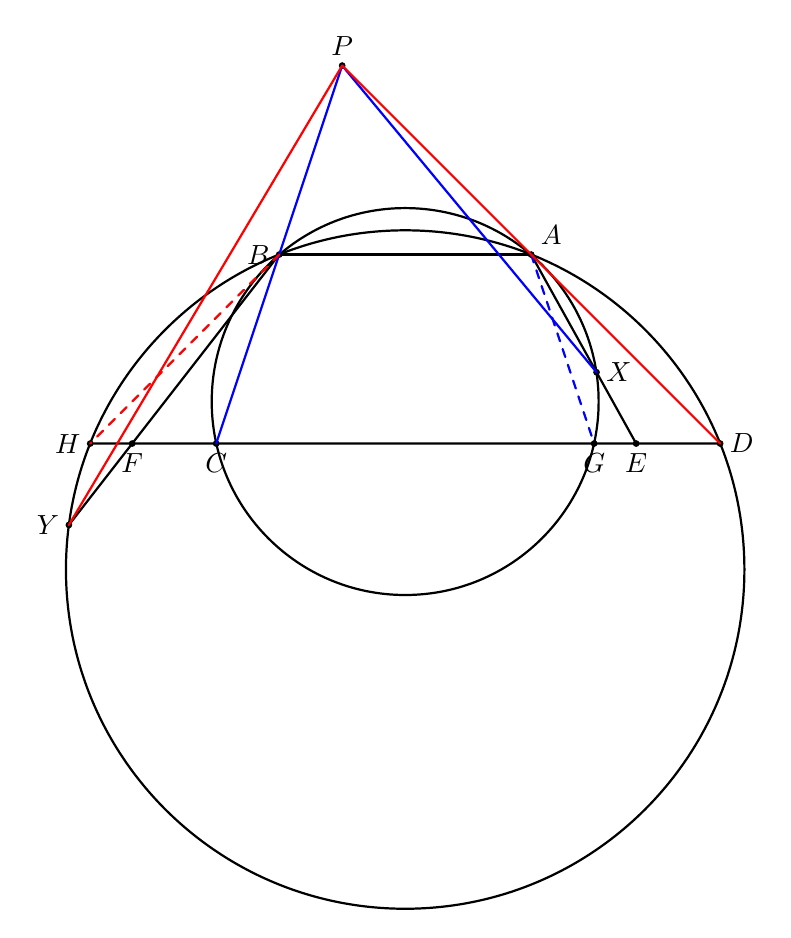
\begin{tikzpicture}[scale=0.8]
    \tkzDefPoint(2,3){A}
    \tkzDefPoint(-2,3){B}
    \tkzDefPoint(-3,0){C}
    \tkzDefPoint(5,0){D}
    \tkzInterLL(A,D)(B,C) \tkzGetPoint{P}
    \tkzCircumCenter(A,B,C) \tkzGetPoint{O_1}
    \tkzCircumCenter(A,B,D) \tkzGetPoint{O_2}
    \tkzInterCC(O_1,C)(P,C) \tkzGetPoints{C_tmp}{X}
    \tkzInterCC(O_2,D)(P,D) \tkzGetPoints{Y}{D_tmp}
    \tkzDrawCircle[black,thick](O_1,A)
    \tkzDrawCircle[black,thick](O_2,A)
    \tkzInterLL(A,X)(C,D) \tkzGetPoint{E}
    \tkzInterLL(B,Y)(C,D) \tkzGetPoint{F}
    \tkzInterLC(C,D)(O_1,A) \tkzGetPoints{C_tmp}{G}
    \tkzInterLC(C,D)(O_2,A) \tkzGetPoints{D_tmp}{H}
    \tkzDrawPoints[fill=black](A,B,C,D,E,F,X,G,H,Y,P)
    \tkzLabelPoints[below](C)
    \tkzLabelPoints[above right](A)
    \tkzLabelPoints[left](B,H)
    \tkzLabelPoints[below](E,F,G)
    \tkzLabelPoints[above](P)
    \tkzLabelPoints[right](X,D)
    \tkzLabelPoints[left](Y)
    \tkzDrawSegments[black, thick](A,B H,D A,E B,Y)
    \tkzDrawSegments[blue, thick](P,C P,X)
    \tkzDrawSegments[dashed, blue, thick](A,G)
    \tkzDrawSegments[dashed, red, thick](B,H)
    \tkzDrawSegments[red, thick](P,Y P,D)
  \end{tikzpicture}
\end{center}
第四步，「長度」轉換成「面積比值」：

留意到$HC=GD$是已知事實，所以要證明命題四，等價於證明$HF$、$GE$分別在$HC$、$GD$內所佔的比值，即等價於以下的命題五：
\begin{equation}
  HF=GE\Leftrightarrow \frac{HC}{HF}=\frac{GD}{GE}\Leftrightarrow\frac{HC}{HF}-1=\frac{GD}{GE}-1\Leftrightarrow\frac{FC}{HF}=\frac{ED}{GE}\label{eq:p2_s5}
\end{equation}
現在觀察$FC/HF$，常用的比值轉換手法就是「長度-面積」，即
\begin{equation}
  \frac{FC}{HF}=\frac{\left[\triangle{CBY}\right]}{\left[\triangle{HBY}\right]}\label{eq:p2_s5-1}
\end{equation}
\begin{center} % 子圖 7
  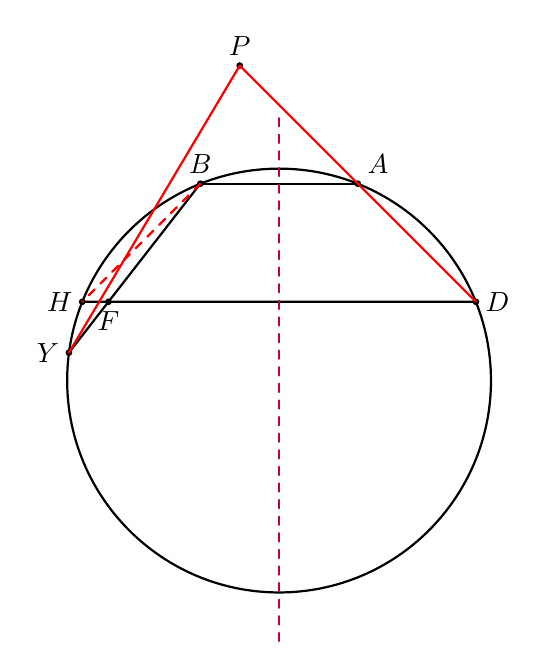
\begin{tikzpicture}[scale=0.5]
    \tkzDefPoint(2,3){A}
    \tkzDefPoint(-2,3){B}
    \tkzDefPoint(-3,0){C}
    \tkzDefPoint(5,0){D}
    \tkzInterLL(A,D)(B,C) \tkzGetPoint{P}
    \tkzCircumCenter(A,B,C) \tkzGetPoint{O_1}
    \tkzCircumCenter(A,B,D) \tkzGetPoint{O_2}
    \tkzInterCC(O_1,C)(P,C) \tkzGetPoints{C_tmp}{X}
    \tkzInterCC(O_2,D)(P,D) \tkzGetPoints{Y}{D_tmp}
    \tkzDrawCircle[black,thick](O_2,A)
    \tkzInterLL(A,X)(C,D) \tkzGetPoint{E}
    \tkzInterLL(B,Y)(C,D) \tkzGetPoint{F}
    \tkzInterLC(C,D)(O_1,A) \tkzGetPoints{C_tmp}{G}
    \tkzInterLC(C,D)(O_2,A) \tkzGetPoints{D_tmp}{H}
    \tkzDrawPoints[fill=black](A,B,D,F,H,Y,P)
    \tkzLabelPoints[above right](A)
    \tkzLabelPoints[left](H)
    \tkzLabelPoints[below](F)
    \tkzLabelPoints[above](P,B)
    \tkzLabelPoints[right](D)
    \tkzLabelPoints[left](Y)
    \tkzDrawSegments[black, thick](A,B H,D B,Y)
    \tkzDrawSegments[dashed, red, thick](B,H)
    \tkzDrawSegments[red, thick](P,Y P,D)
    \tkzDrawLine[purple, thick, dashed, add=1.5 and 2.5](O_1,O_2)
  \end{tikzpicture}
\end{center}
前面的部分有提及「線段$BA$和$HD$被同一條直線垂直平分」，所以有
\begin{equation}
  \begin{aligned}
    \text{（中垂線）軸對稱：}&B\rightarrow A\\
    &H\rightarrow D
  \end{aligned}
  \quad\Rightarrow\quad BH=AD\label{eq:p2_s5-2}
\end{equation}
\begin{center} % 子圖 8
  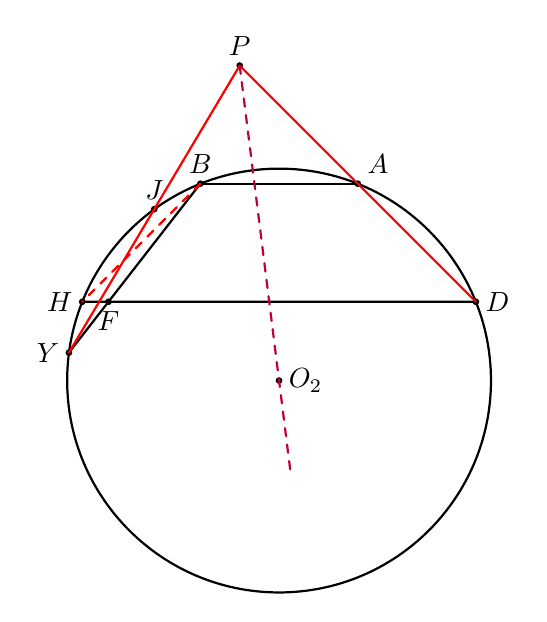
\begin{tikzpicture}[scale=0.5]
    \tkzDefPoint(2,3){A}
    \tkzDefPoint(-2,3){B}
    \tkzDefPoint(-3,0){C}
    \tkzDefPoint(5,0){D}
    \tkzInterLL(A,D)(B,C) \tkzGetPoint{P}
    \tkzCircumCenter(A,B,C) \tkzGetPoint{O_1}
    \tkzCircumCenter(A,B,D) \tkzGetPoint{O_2}
    \tkzInterCC(O_1,C)(P,C) \tkzGetPoints{C_tmp}{X}
    \tkzInterCC(O_2,D)(P,D) \tkzGetPoints{Y}{D_tmp}
    \tkzDrawCircle[black,thick](O_2,A)
    \tkzInterLL(A,X)(C,D) \tkzGetPoint{E}
    \tkzInterLL(B,Y)(C,D) \tkzGetPoint{F}
    \tkzInterLC(C,D)(O_1,A) \tkzGetPoints{C_tmp}{G}
    \tkzInterLC(C,D)(O_2,A) \tkzGetPoints{D_tmp}{H}
    \tkzInterLC(P,Y)(O_2,A) \tkzGetPoints{J}{Y_tmp}
    \tkzDrawPoints[fill=black](A,B,D,F,H,Y,P,O_2,J)
    \tkzLabelPoints[above right](A)
    \tkzLabelPoints[left](H)
    \tkzLabelPoints[below](F)
    \tkzLabelPoints[above](P,B,J)
    \tkzLabelPoints[right](D,O_2)
    \tkzLabelPoints[left](Y)
    \tkzDrawSegments[black, thick](A,B H,D B,Y)
    \tkzDrawSegments[dashed, red, thick](B,H)
    \tkzDrawSegments[red, thick](P,Y P,D)
    \tkzDrawLine[purple, thick, dashed, add=0 and 0.3](P,O_2)
  \end{tikzpicture}
\end{center}  
熟悉尺規作圖的讀者亦必然發現，$Y$點是$D$點關於「$P$點與$\triangle{ABD}$外心的連線」對稱的。作$\triangle{ABD}$外心為$O_2$，有
\begin{align*}
  \text{（$PO_2$）軸對稱：}&A\rightarrow ??\\
  &D\rightarrow Y
\end{align*}
顯然「??」是$PY$與$\triangle{ABD}$外接圓且異於$Y$的另一個交點，記為$J$。由兩割線定理可知
\begin{equation}
  PA=PJ,AD=JY\label{eq:p2_s5-2A}
\end{equation}
現時有結論如下：
\begin{equation}
  BH=AD=JY\label{eq:p2_s5-3}
\end{equation}
由圓周角定理可知
\begin{equation}
  \text{劣弧}HB=\text{劣弧}AD=\text{劣弧}YJ\quad\Rightarrow\quad\text{劣弧}YH=\text{劣弧}BJ\quad\Rightarrow\quad YH=BJ\label{eq:p2_s5-4}
\end{equation}
由(\ref{eq:p2_s5-3})和(\ref{eq:p2_s5-4})可知，$\triangle{HBY}\cong\triangle{JYB}$。所以(\ref{eq:p2_s5-1})式等價於
\begin{equation}
  \frac{FC}{HF}=\frac{\left[\triangle{CBY}\right]}{\left[\triangle{JYB}\right]}\label{eq:p2_s5-5}
\end{equation}
同理，作$PX$與$\triangle{ABC}$外接圓且異於$X$的另一個交點，記為$I$，亦有
\begin{equation}
  \frac{ED}{GE}=\frac{\left[\triangle{DAX}\right]}{\left[\triangle{IXA}\right]}\label{eq:p2_s5-6}
\end{equation}
所以要證明命題五等價於以下的命題六：
\begin{equation}
  \frac{\left[\triangle{CBY}\right]}{\left[\triangle{JYB}\right]}=\frac{\left[\triangle{DAX}\right]}{\left[\triangle{IXA}\right]}\label{eq:p2_s6}
\end{equation}
整理當前幾何圖
\begin{center} % 子圖 9
  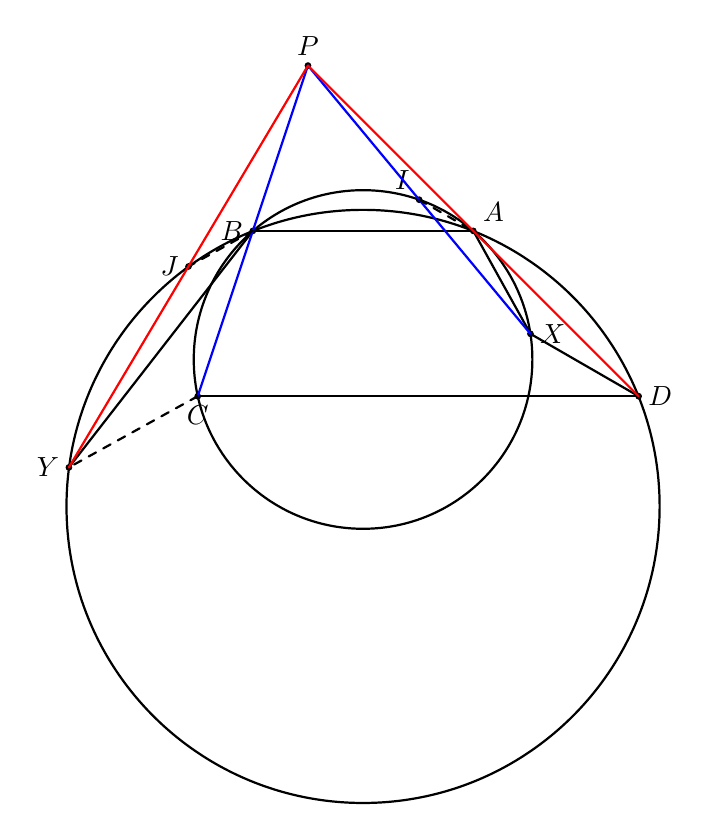
\begin{tikzpicture}[scale=0.7]
    \tkzDefPoint(2,3){A}
    \tkzDefPoint(-2,3){B}
    \tkzDefPoint(-3,0){C}
    \tkzDefPoint(5,0){D}
    \tkzInterLL(A,D)(B,C) \tkzGetPoint{P}
    \tkzCircumCenter(A,B,C) \tkzGetPoint{O_1}
    \tkzCircumCenter(A,B,D) \tkzGetPoint{O_2}
    \tkzInterCC(O_1,C)(P,C) \tkzGetPoints{C_tmp}{X}
    \tkzInterCC(O_2,D)(P,D) \tkzGetPoints{Y}{D_tmp}
    \tkzDrawCircle[black,thick](O_1,A)
    \tkzDrawCircle[black,thick](O_2,A)
    \tkzInterLL(A,X)(C,D) \tkzGetPoint{E}
    \tkzInterLL(B,Y)(C,D) \tkzGetPoint{F}
    \tkzInterLC(C,D)(O_1,A) \tkzGetPoints{C_tmp}{G}
    \tkzInterLC(C,D)(O_2,A) \tkzGetPoints{D_tmp}{H}
    \tkzInterLC(P,Y)(O_2,A) \tkzGetPoints{J}{Y_tmp}
    \tkzInterLC(P,X)(O_1,A) \tkzGetPoints{X_tmp}{I}
    \tkzDrawPoints[fill=black](A,B,C,D,X,Y,P,I,J)
    \tkzLabelPoints[below](C)
    \tkzLabelPoints[above right](A)
    \tkzLabelPoints[above left](I)
    \tkzLabelPoints[left](B,J)
    \tkzLabelPoints[above](P)
    \tkzLabelPoints[right](X,D)
    \tkzLabelPoints[left](Y)
    \tkzDrawSegments[black, thick](A,B X,D A,X B,Y C,D)
    \tkzDrawSegments[blue, thick](P,C P,X)
    \tkzDrawSegments[dashed, black, thick](B,J I,A C,Y)
    \tkzDrawSegments[red, thick](P,Y P,D)
  \end{tikzpicture}
\end{center}
第六步，「面積比值」轉化成「長度比值」：
\begin{align}
  \frac{\left[\triangle{CBY}\right]}{\left[\triangle{JYB}\right]}
  &=\frac{\left[\triangle{CBY}\right]/\left[\triangle{PBY}\right]}{\left[\triangle{JYB}\right]/\left[\triangle{PYB}\right]}\notag\\
  &=\frac{CB/BP}{JY/PY}\notag\\
  &=\frac{CB/BP}{AD/PD}\label{eq:p2_s6-1}
\end{align}
同理可得
\begin{equation}
  \frac{\left[\triangle{DAX}\right]}{\left[\triangle{IXA}\right]}=\frac{DA/AP}{BC/PC}\label{eq:p2_s6-2}
\end{equation}
由「平行線分線段成比例」可知
\begin{align}
  CB/BP&=DA/AP\\
  AD/PD&=BC/PC
\end{align}
由此可得
\begin{equation}
  \frac{\left[\triangle{CBY}\right]}{\left[\triangle{JYB}\right]}=\frac{CB/BP}{AD/PD}=\frac{DA/AP}{BC/PC}=\frac{\left[\triangle{DAX}\right]}{\left[\triangle{IXA}\right]}\label{eq:p2_s6-3}
\end{equation}
命題六成立，即原命題得證。
%================ Solution 2 ================%
\newpage
%================ Problem 3 ================%
\INDEX{問題3}滿足下列條件 (i) 和 (ii) 的有限長實數列 $\left\{a_n\right\}_{n=1}^{m}\left(m\geq10\right)$ 是一個 $m$-有趣數列：
\begin{enumerate}[label = (\roman*)]
  \item 對任意 $k=1,2,\cdots,m-1$，都有 $\left|a_{k+1}-a_k\right|=1$；
  \item 存在正整數 $i_1,i_2,\cdots,i_{10}\left(i_1<i_2<\cdots<i_{10}\leq m\right)$，使得 $\left\{a_{i_k}\right\}_{k=1}^{10}$ 是等比數列，且該等比數列的公比 $q\neq\pm1$。
\end{enumerate}
記 $m_0$ 為使得 $m$-有趣數列存在的最小正整數 $m$。求 $m_0$ 的值，並確定不同的 $m_0$-有趣數列的個數。
%================ Problem 3 ================%
\newpage
%================ Solution 3 ================%
\INDEX{證明：}\setcounter{equation}{0}
首先，留意到 $m_0$ 具有「最小性」，所以我們要知道，\textbf{極端性原理}將會是解題的關鍵方式。
\begin{quotation}
  極端性原理通俗來說，就是「如果是 $X$ 是最大（小）的，那麼其他數 $y$ 都不可能比 $X$ 大（小）。」
\end{quotation}
然後，我們要嘗試描繪這個 $m_0$-有趣數列的「形狀」——盡可能找出把這個數列的特徵，
這個過程必須要善用反證法和極端性原理。

\textbf{第一步：}我們要觀察數列的「頭」和「尾」：
取一個 $m_0$-有趣數列 $\left\{a_n\right\}_{n=1}^{m_0}$，

如果 $i_1>1$ 或 $i_{10}<m_0$，我們可以觀察「紅色」的子數列： 
\begin{equation*}
  a_1,a_2,\cdots,\color{red}{a_{i_1},a_{i_1+1},\cdots,a_{i_2},a_{i_2+1},\cdots,a_{i_{10}}}\color{black}{,a_{i_{10}+1},\cdots,a_{m_0}}
\end{equation*}
數列$\left\{a_n\right\}_{n=i_1}^{i_{10}}$顯然也滿足條件 (i) 和 (ii)，
但是數列長度為 $i_{10}-i_1+1<m_0$，與 $m_0$ 的最小性矛盾。

由此可得出\textbf{結論一：}\fbox{$m_0$-有趣數列必須滿足 $i_1=1$ 且 $i_{10}=m_0$}，剪去了有趣數列的「頭」和「尾」。

\textbf{第二步：}我們要觀察數列的「節」：觀察 $m_0$-有趣數列 $\left\{a_n\right\}_{n=1}^{m_0}$ 的中間部分
$$
  a_{i_k},\color{red}{a_{i_k+1},a_{i_k+2},\cdots,a_{i_{k+1}-1}}\color{black}{,a_{i_{k+1}}}
$$
紅色部分有 $i_{k+1}-i_k-1$ 個元素。利用條件 (i) 可以得到以下神奇的變換：
\begin{equation}
  i_{k+1}-i_k=\sum_{j=i_k}^{i_{k+1}-1}{1}=\sum_{j=i_k}^{i_{k+1}-1}{\left|a_{j+1}-a_j\right|}\geq\left|\sum_{j=i_k}^{i_{k+1}-1}{\left(a_{j+1}-a_j\right)}\right|=|a_{i_{k+1}}-a_{i_k}|\label{eq:p3_s1}
\end{equation}
不等式 (\ref{eq:p3_s1}) 的等號成立的條件是所有 $a_{j+1}-a_j$ 同號，
即子數列$\left\{a_j\right\}_{j=i_k}^{i_{k+1}}$嚴格單調遞增或遞減（以下統稱「嚴格單調」）。

相反，如果子數列$\left\{a_j\right\}_{j=i_k}^{i_{k+1}}$不是嚴格單調的，
則不等式 (\ref{eq:p3_s1}) 中的「$\geq$」直接變成「$>$」。這意味着我們可以把「紅色」子數列按照以下的情況替換成「藍色」子數列：
\begin{itemize}
  \item 如果 $a_{i_k}<a_{i_{k+1}}$，則「藍色」子數列為$a_{i_k},\color{blue}{a_{i_k}+1,a_{i_k}+2,\cdots,a_{i_{k+1}}-1}\color{black}{,a_{i_{k+1}}}$
  \item 如果 $a_{i_k}>a_{i_{k+1}}$，則「藍色」子數列為$a_{i_k},\color{blue}{a_{i_k}-1,a_{i_k}-2,\cdots,a_{i_{k+1}}+1}\color{black}{,a_{i_{k+1}}}$
\end{itemize}
此時得到另一個數列 $a_1,a_2,\cdots,a_{i_k},\color{blue}{a_{i_k}\pm1,a_{i_k}\pm2,\cdots,a_{i_{k+1}}\mp1}\color{black}{,a_{i_{k+1}},a_{i_{k+1}+1},\cdots,a_{m_0}}$，
亦滿足條件 (i) 和 (ii)，但是數列長度比 $m_0$ 短 $i_{k+1}-i_k-|a_{i_{k+1}}-a_{i_k}|>0$，與 $m_0$ 的最小性矛盾。

由此可得出\textbf{結論二：}\fbox{$m_0$-有趣數列$\left\{a_n\right\}_{n=1}^{m_0}$的子數列$\left\{a_j\right\}_{j=i_k}^{i_{k+1}}$必須嚴格單調，即是公差為 $\pm1$ 的等差數列}。

\textbf{第三步：}我們要考察$m_0$-有趣數列的等比子數列$\left\{a_{i_k}\right\}_{k=1}^{10}$的公比 $q$ ：

利用合比定理可知
\begin{equation}
  q=\frac{a_{i_3}}{a_{i_2}}=\frac{a_{i_2}}{a_{i_1}}=\frac{a_{i_3}-a_{i_2}}{a_{i_2}-a_{i_1}}\label{eq:p3_s2}
\end{equation}
第二步的推論如下：
\begin{equation}
  \left|a_{i_{k+1}}-a_{i_k}\right|=i_{k+1}-i_k,\ k=1,2,\cdots,9\label{eq:p3_s3}
\end{equation}
結合(\ref{eq:p3_s3})可知
\begin{equation}
  |q|=\left|\frac{a_{i_3}-a_{i_2}}{a_{i_2}-a_{i_1}}\right|=\frac{i_3-i_2}{i_2-i_1}\in\mathbb{Q}\label{eq:p3_s4}
\end{equation}
再由(\ref{eq:p3_s3})可知
\begin{equation}
  |a_1\left(q-1\right)|=|a_{i_2}-a_{i_1}|=i_2-i_1\in\mathbb{Z}^+\label{eq:p3_s5}
\end{equation}
由此可得出\textbf{結論三：}\fbox{公比 $q$ 是有理數且 $\left|a_1\left(q-1\right)\right|$ 是正整數}。

\textbf{第四步：}我們可以先做計算一次 $m_0$ ：

利用第一步的結論、第二步的推論和等比數列通項公式可知
\begin{align}
  m_0&=1+m_0-1\notag\\
  &=1+i_{10}-i_1\tag{第一步的結論}\\
  &=1+\sum_{k=1}^{9}{\left(i_{k+1}-i_k\right)}\notag\\
  &=1+\sum_{k=1}^{9}{\left|a_{i_{k+1}}-a_{i_k}\right|}\tag{第二步的推論}\\
  &=1+\left|q-1\right|\sum_{k=1}^{9}{|a_{i_k}|}\notag\\
  &=1+\left|a_1\left(q-1\right)\right|\sum_{k=1}^{9}{|q|^{k-1}}\label{eq:p3_s6}
\end{align}
既然 $m_0$ 具有最小性，我們必須規限 $\left|a_1\left(q-1\right)\right|$ 和 $|q|$ 的下界。

容易得知，如果我們把 $m_0$-有趣數列 $\left\{a_n\right\}_{n=1}^{m_0}$進行「倒序」操作
$$
  b_n=a_{m_0+1-n},\ n=1,2,\cdots,m_0
$$
得到的數列 $\left\{b_n\right\}_{n=1}^{m_0}$ 也是 $m_0$-有趣的，其中的等比子數列 $\left\{b_{j_k}\right\}_{k=1}^{10}=\left(a_{i_{10}},a_{i_9},\cdots,a_{i_1}\right)$ 的公比 $q_b = 1/q$。
由此可知，$\left\{a_n\right\}_{n=1}^{m_0}$ 及其倒序數列 $\left\{b_n\right\}_{n=1}^{m_0}=\left\{a_{m_0+1-n}\right\}_{n=1}^{m_0}$ 的等比子數列之公比絕對值 $|q|$ 和 $|q_b|$ 之間，有且只有一個小於1。

不妨假設 $|q|<1$，配合結論三可設 $|q|=M/N$，其中 $M,N\in\mathbb{Z}^+$，$M<N$ 且 $\gcd\left(M,N\right)=1$。

再由式(\ref{eq:p3_s3})及等比數列的通項公式可知
\begin{equation}
  i_{10}-i_9=\left|a_{i_{10}}-a_{i_9}\right|=\left|a_1\left(q-1\right)\right|\left|q\right|^8=\frac{\left|a_1\left(1-q\right)\right|M^8}{N^8}\ \Rightarrow\ N^8\left|\left[a_1\left(1-q\right)\right]M^8\right.
\end{equation}
因為 $\gcd\left(M,N\right)=1$，所以有 $N^8|a_1\left(1-q\right)$，記 $K=\dfrac{\left|a_1\left(1-q\right)\right|}{N^8}\in\mathbb{Z}^+$，那麼(\ref{eq:p3_s6})可改寫成
\begin{align}
  m_0&=1+\left|a_1\left(q-1\right)\right|\sum_{k=1}^{9}{\frac{M^{k-1}}{N^{k-1}}}\notag\\
  &=1+\frac{\left|a_1\left(q-1\right)\right|}{N^8}\sum_{k=1}^{9}{\frac{M^{k-1}N^8}{N^{k-1}}}\notag\\
  &=1+K\sum_{k=1}^{9}{M^{k-1}N^{9-k}}\notag\\
  &\geq1+1\times\sum_{k=1}^{9}{M^{k-1}\left(M+1\right)^{9-k}}\notag\\
  &\geq1+\sum_{k=1}^{9}{1^{k-1}\left(1+1\right)^{9-k}}\notag\\
  &=2^9\label{eq:p3_s7}
\end{align}
式(\ref{eq:p3_s7})的等號成立條件是 $K=M=1$ 且 $N=M+1=2$，此時 $|q|=1/2$，$|a_1\left(1-q\right)|=2^8$，此表示以下四組的等號成立條件：
\begin{equation}
  \left\{\begin{matrix}
    q=1/2\\
    a_1=2^9
  \end{matrix}\right.\ 
  \left\{\begin{matrix}
    q=1/2\\
    a_1=-2^9
  \end{matrix}\right.\ 
  \left\{\begin{matrix}
    q=-1/2\\
    a_1=2^9/3
  \end{matrix}\right.\ 
  \left\{\begin{matrix}
    q=-1/2\\
    a_1=-2^9/3
  \end{matrix}\right.
\end{equation}
第一組等號成立條件可以得到的有趣數列是 $a_n=513-n, n=1,2,\cdots,512$；

第二組等號成立條件可以得到的有趣數列是 $a_n=-513+n, n=1,2,\cdots,512$；

第三組等號成立條件可以得到的有趣數列是
\begin{table}[htbp]
  \small
  \setlength{\tabcolsep}{4pt}
  \centering
  \begin{tabular}{cccccccccccccccccc}
    $\dfrac{2^9}{3}$&($\color{red}\bigstar$\tablefootnote{$\color{red}\bigstar$為公差為 $-1$ 的等差數列})&$-\dfrac{2^8}{3}$&($\color{blue}\bigstar$\tablefootnote{$\color{blue}\bigstar$為公差為 $1$ 的等差數列})&$\dfrac{2^7}{3}$&($\color{red}\bigstar$)&$-\dfrac{2^6}{3}$&($\color{blue}\bigstar$)&$\dfrac{2^5}{3}$&($\color{red}\bigstar$)&$-\dfrac{2^4}{3}$&($\color{blue}\bigstar$)&$\dfrac{2^3}{3}$&($\color{red}\bigstar$)&$-\dfrac{2^2}{3}$&($\color{blue}\bigstar$)&$\dfrac{2^1}{3}$&$-\dfrac{2^0}{3}$\\
    \hline
    $a_1$&$\cdots$&$a_{257}$&$\cdots$&$a_{385}$&$\cdots$&$a_{449}$&$\cdots$&$a_{481}$&$\cdots$&$a_{497}$&$\cdots$&$a_{505}$&$\cdots$&$a_{509}$&$\cdots$&$a_{511}$&$a_{512}$
  \end{tabular}
\end{table}\\
第四組等號成立條件可以得到的有趣數列是
\begin{table}[htbp]
  \small
  \setlength{\tabcolsep}{4pt}
  \centering
  \begin{tabular}{cccccccccccccccccc}
    $-\dfrac{2^9}{3}$&($\color{blue}\bigstar$)&$\dfrac{2^8}{3}$&($\color{red}\bigstar$)&$-\dfrac{2^7}{3}$&($\color{blue}\bigstar$)&$\dfrac{2^6}{3}$&($\color{red}\bigstar$)&$-\dfrac{2^5}{3}$&($\color{blue}\bigstar$)&$\dfrac{2^4}{3}$&($\color{red}\bigstar$)&$-\dfrac{2^3}{3}$&($\color{blue}\bigstar$)&$\dfrac{2^2}{3}$&($\color{red}\bigstar$)&$-\dfrac{2^1}{3}$&$\dfrac{2^0}{3}$\\
    \hline
    $a_1$&$\cdots$&$a_{257}$&$\cdots$&$a_{385}$&$\cdots$&$a_{449}$&$\cdots$&$a_{481}$&$\cdots$&$a_{497}$&$\cdots$&$a_{505}$&$\cdots$&$a_{509}$&$\cdots$&$a_{511}$&$a_{512}$
  \end{tabular}
\end{table}\\
以上四個數列的「倒序」數列也是 512-有趣數列，而且這八個數列兩兩不同。

\fbox{因此，題中所求的 $m_0$ 為 512，對應不同的 $m_0$-有趣數列共有 8 個。}
%================ Solution 3 ================%
\newpage
%================ Problem 4 ================%
\INDEX{問題4}不等邊銳角 $\triangle{ABC}$ 的外心為 $O$，
由 $A$ 點向 $BC$ 的垂線的垂足為 $D$，
$P$ 點在直線 $AO$ 上且不在 $\triangle{ABC}$ 的外接圓上。
以線段 $AP$ 為直徑的圓$\Gamma$，與 $\triangle{BCP}$ 的外接圓相交於 $E\neq P$，
與平行於 $BC$ 且過 $A$ 的直線相交於 $F\neq A$。

\textbf{求證：}$D$、$E$ 和 $F$ 三點共線。
\begin{figure}[htbp] % p4 示意圖
  \centering
  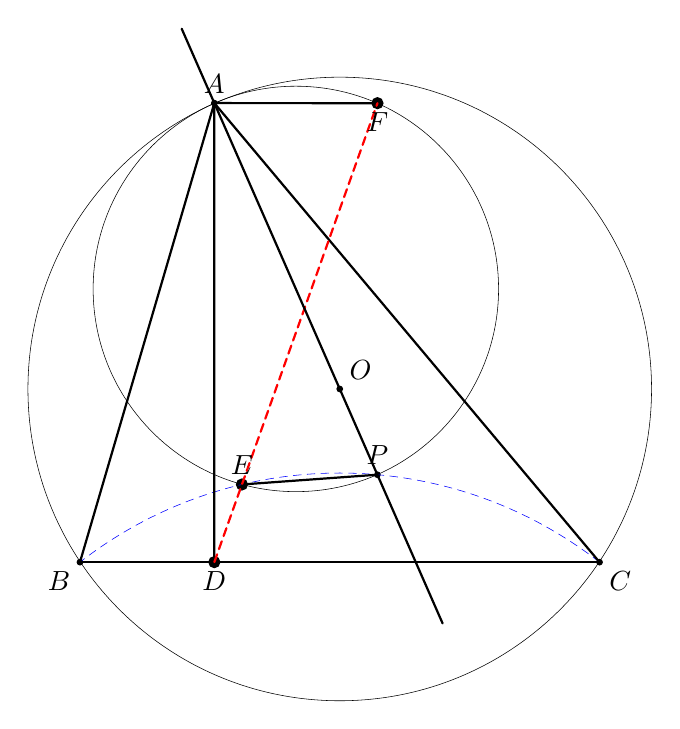
\begin{tikzpicture}[scale=1.1]
    \tkzDefPoints{0/0/O, -3/-2/B, 3/-2/C}
    \tkzDefPointBy[rotation=center O angle -100](B)\tkzGetPoint{A}
    \tkzDefPointBy[projection=onto B--C](A)\tkzGetPoint{D}
    \tkzDefPointWith[linear, K=1.3](A,O)\tkzGetPoint{P}
    \tkzDefPointWith[linear, K=0.5](A,P)\tkzGetPoint{X}
    \tkzDefCircle[circum](B,P,C)\tkzGetPoint{O1}
    \tkzInterCC[common=P](X,P)(O1,P)\tkzGetFirstPoint{E}
    \tkzDefLine[parallel=through A](B,C)\tkzGetPoint{L}
    \tkzInterLL(A,L)(D,E)\tkzGetPoint{F}
    \tkzDrawPoints[black](A,B,C,P,O)
    \tkzDrawPoints[size=4, fill=black](D,E,F)
    \tkzDrawCircle[black](O,B)
    \tkzDrawCircle[black](X,A)
    \tkzDrawArc[blue, densely dashed](O1,C)(B)
    \tkzDrawSegments[black, thick](A,B A,C B,C A,D P,E A,F)
    \tkzDrawSegment[red, thick, densely dashed](D,F)
    \tkzDrawLine[black, thick, add=0.2 and 0.4](A,P)
    \tkzLabelPoints[above](A,E,P)
    \tkzLabelPoints[below left](B)
    \tkzLabelPoints[below right](C)
    \tkzLabelPoints[below](D,F)
    \tkzLabelPoints[above right](O)
  \end{tikzpicture}
\end{figure}
%================ Problem 4 ================%
\newpage
%================ Solution 4 ================%
\INDEX{證明：}\INDEX{證明：}\setcounter{equation}{0}
因為 $A$、$F$、$P$、$E$ 四點共圓，所以直線對（pair） $\left(AF,PE\right)$ 關於直線對 $\left(AP,EF\right)$ 反平行。

因為 $AF // BC$，所以直線對 $\left(BC,PE\right)$ 關於直線對 $\left(AP,EF\right)$ 反平行。

因此原命題按如下方式進行等價變換，變換後的命題稱為命題一：
\begin{equation}
  \text{$D$、$E$ 和 $F$ 三點共線}\ \Leftrightarrow\ \measuredangle{\left(DE,EF\right)}=0^{\circ}\ \Leftrightarrow\ \text{直線對 $\left(BC,PE\right)$ 關於直線對 $\left(AP,DE\right)$ 反平行}
\end{equation}
此時完全消去了 $F$ 點，整理幾何圖如下：

\begin{figure}[htbp] % 子圖 1
  \centering
  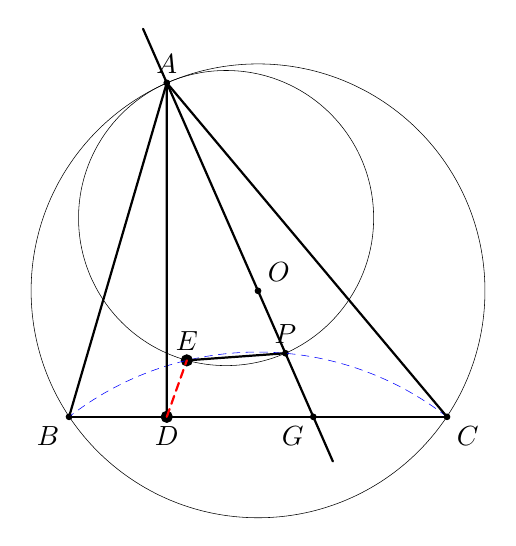
\begin{tikzpicture}[scale=0.8]
    \tkzDefPoints{0/0/O, -3/-2/B, 3/-2/C}
    \tkzDefPointBy[rotation=center O angle -100](B)\tkzGetPoint{A}
    \tkzDefPointBy[projection=onto B--C](A)\tkzGetPoint{D}
    \tkzDefPointWith[linear, K=1.3](A,O)\tkzGetPoint{P}
    \tkzDefPointWith[linear, K=0.5](A,P)\tkzGetPoint{X}
    \tkzDefCircle[circum](B,P,C)\tkzGetPoint{O1}
    \tkzInterCC[common=P](X,P)(O1,P)\tkzGetFirstPoint{E}
    \tkzInterLL(A,O)(B,C)\tkzGetPoint{G}
    %\tkzDefLine[parallel=through A](B,C)\tkzGetPoint{L}
    %\tkzInterLL(A,L)(D,E)\tkzGetPoint{F}
    \tkzDrawPoints[black](A,B,C,P,O,G)
    \tkzDrawPoints[size=4, fill=black](D,E)
    \tkzDrawCircle[black](O,B)
    \tkzDrawCircle[black](X,A)
    \tkzDrawArc[blue, densely dashed](O1,C)(B)
    \tkzDrawSegments[black, thick](A,B A,C B,C A,D P,E)
    \tkzDrawSegment[red, thick, densely dashed](D,E)
    \tkzDrawLine[black, thick, add=0.2 and 0.4](A,P)
    \tkzLabelPoints[above](A,E,P)
    \tkzLabelPoints[below left](B,G)
    \tkzLabelPoints[below right](C)
    \tkzLabelPoints[below](D)
    \tkzLabelPoints[above right](O)
  \end{tikzpicture}
\end{figure}
設 $AO$ 交 $BC$ 於 $G$，命題一可以按如下方式進行等價變換，變換後的命題稱為命題二：
\begin{equation}
  (1)\ \Leftrightarrow\ \text{直線對 $\left(DG,PE\right)$ 關於直線對 $\left(PG,DE\right)$ 反平行}\ \Leftrightarrow\ \text{$D$、$E$、$P$、$G$ 四點共圓}
\end{equation}

\begin{figure}[htbp] % 子圖 2
  \centering
  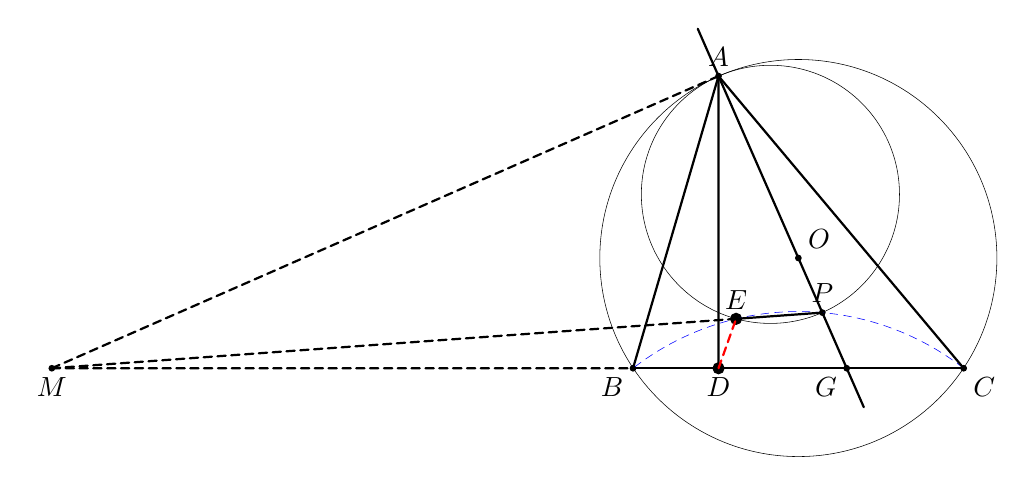
\begin{tikzpicture}[scale=0.7]
    \tkzDefPoints{0/0/O, -3/-2/B, 3/-2/C}
    \tkzDefPointBy[rotation=center O angle -100](B)\tkzGetPoint{A}
    \tkzDefPointBy[projection=onto B--C](A)\tkzGetPoint{D}
    \tkzDefPointWith[linear, K=1.3](A,O)\tkzGetPoint{P}
    \tkzDefPointWith[linear, K=0.5](A,P)\tkzGetPoint{X}
    \tkzDefCircle[circum](B,P,C)\tkzGetPoint{O1}
    \tkzInterCC[common=P](X,P)(O1,P)\tkzGetFirstPoint{E}
    \tkzInterLL(A,O)(B,C)\tkzGetPoint{G}
    \tkzInterLL(P,E)(B,C)\tkzGetPoint{M}
    %\tkzDefLine[parallel=through A](B,C)\tkzGetPoint{L}
    %\tkzInterLL(A,L)(D,E)\tkzGetPoint{F}
    \tkzDrawPoints[black](A,B,C,P,O,G,M)
    \tkzDrawPoints[size=4, fill=black](D,E)
    \tkzDrawCircle[black](O,B)
    \tkzDrawCircle[black](X,A)
    \tkzDrawArc[blue, densely dashed](O1,C)(B)
    \tkzDrawSegments[black, thick](A,B A,C B,C A,D P,E)
    \tkzDrawSegments[black, thick, densely dashed](M,B M,E M,A)
    \tkzDrawSegment[red, thick, densely dashed](D,E)
    \tkzDrawLine[black, thick, add=0.2 and 0.4](A,P)
    \tkzLabelPoints[above](A,E,P)
    \tkzLabelPoints[below left](B,G)
    \tkzLabelPoints[below right](C)
    \tkzLabelPoints[below](D,M)
    \tkzLabelPoints[above right](O)
  \end{tikzpicture}
\end{figure}
設 $PE$ 交 $DG$ 於 $M$，命題二可由圓冪定理等價變換成命題三：
\begin{equation}
  (2) \Leftrightarrow\ \overrightarrow{MP}\cdot\overrightarrow{ME}=\overrightarrow{MD}\cdot\overrightarrow{MG}
\end{equation}
因為 $DG$ 和 $BC$ 為同一直線，所以 $M$ 也是 $PE$ 和 $BC$ 的交點。

注意到，$PE$ 是圓 $\Gamma$ 和 $\triangle{BPC}$ 外接圓的根軸，
$BC$ 是 $\triangle{BPC}$ 外接圓及 $\triangle{ABC}$ 外接圓的根軸，
所以由根心定理可知 $M$ 點便是圓 $\Gamma$、$\triangle{BPC}$ 外接圓和$\triangle{ABC}$ 外接圓的根心。

顯然，圓 $\Gamma$ 和 $\triangle{ABC}$ 外接圓相切於 $A$ 點，
所以圓 $\Gamma$ 和 $\triangle{ABC}$ 外接圓的根軸就是通過 $A$ 點的切線。
由根心定理可知，$MA$ 便是上述的切線。利用圓冪定理可得 $\overrightarrow{MP}\cdot\overrightarrow{ME}=MA^2$，命題三便可以等價變換成命題四：
\begin{equation}
  (3)\ \Leftrightarrow\ MA^2=\overrightarrow{MD}\cdot\overrightarrow{MG}
\end{equation}
此時完全消去了 $E$ 和 $P$ 點，整理幾何圖如下：

\begin{figure}[htbp] % 子圖 3
  \centering
  \begin{tikzpicture}[scale=0.7]
    \tkzDefPoints{0/0/O, -3/-2/B, 3/-2/C}
    \tkzDefPointBy[rotation=center O angle -100](B)\tkzGetPoint{A}
    \tkzDefPointBy[projection=onto B--C](A)\tkzGetPoint{D}
    \tkzDefPointWith[linear, K=1.3](A,O)\tkzGetPoint{P}
    %\tkzDefPointWith[linear, K=0.5](A,P)\tkzGetPoint{X}
    %\tkzDefCircle[circum](B,P,C)\tkzGetPoint{O1}
    \tkzInterCC[common=P](X,P)(O1,P)\tkzGetFirstPoint{E}
    \tkzInterLL(A,O)(B,C)\tkzGetPoint{G}
    \tkzInterLL(P,E)(B,C)\tkzGetPoint{M}
    %\tkzDefLine[parallel=through A](B,C)\tkzGetPoint{L}
    %\tkzInterLL(A,L)(D,E)\tkzGetPoint{F}
    \tkzDrawPoints[black](A,B,C,O,G,M)
    \tkzDrawPoints[size=4, fill=black](D)
    \tkzDrawCircle[black](O,B)
    %\tkzDrawCircle[black](X,A)
    %\tkzDrawArc[blue, densely dashed](O1,C)(B)
    \tkzDrawSegments[black, thick](A,B A,C B,C A,D A,G)
    \tkzDrawSegments[black, thick, densely dashed](M,B M,A)
    %\tkzDrawSegment[red, thick, densely dashed](D,E)
    %\tkzDrawLine[black, thick, add=0.2 and 0.4](A,P)
    \tkzLabelPoints[above](A)
    \tkzLabelPoints[below left](B,G)
    \tkzLabelPoints[below right](C)
    \tkzLabelPoints[below](D,M)
    \tkzLabelPoints[above right](O)
    \tkzMarkRightAngle[color=blue, size=0.6, line width=2pt](M,A,G)
  \end{tikzpicture}
\end{figure}
因為 $MA$ 是$\triangle{ABC}$ 外接圓的切線，所以 $MA\perp AO$，即 $MA\perp AG$，由此可知 $\triangle{MAG}$ 是直角三角形，斜邊為 $MG$。

因為 $AD\perp BC$，所以 $AD\perp MG$，即 $AD$ 是直角 $\triangle{MAG}$ 斜邊上的高，由射影定理可知
\begin{equation}
  MA^2=\overrightarrow{MD}\cdot\overrightarrow{MG}
\end{equation}
因為命題四成立，且以上每步命題變換均為等價的，所以原命題得證。
%================ Solution 4 ================%
\newpage
%================ Problem 5 ================%
\INDEX{問題5}\INDEX{問題 5}$\triangle{ABC}$ 的重心為 $G$，$R$ 和 $S$ 分別在射線 $GB$ 和 $GC$ 上，且滿足
$$
  \angle{ABS}=\angle{ACR}=180^{\circ}-\angle{BGC}
$$
\textbf{求證：}$\angle{RAS}+\angle{BAC}=\angle{BGC}$。
\begin{figure}[htbp] % p5 示意圖
  \centering
  \begin{tikzpicture}[scale=1.1]
    \tkzDefPoints{-0.5/7/A, -2/0/B, 3/0/C}
    \tkzDefTriangleCenter[centroid](A,B,C)\tkzGetPoint{G}
    \tkzDefLine[orthogonal=through B](A,B)\tkzGetPoint{X1}
    \tkzDefLine[mediator](G,B)\tkzGetPoints{X2}{X3}
    \tkzInterLL(B,X1)(X2,X3)\tkzGetPoint{O_B}
    \tkzInterLC[common=G](G,C)(O_B,G)\tkzGetFirstPoint{S}
    \tkzDefLine[orthogonal=through C](A,C)\tkzGetPoint{Y1}
    \tkzDefLine[mediator](G,C)\tkzGetPoints{Y2}{Y3}
    \tkzInterLL(C,Y1)(Y2,Y3)\tkzGetPoint{O_C}
    \tkzInterLC[common=G](G,B)(O_C,G)\tkzGetFirstPoint{R}
    \tkzDrawPoints[black](A,B,C,G,R,S)
    \tkzDrawSegments[black, thick](A,B A,C B,C G,R G,S B,S C,R)
    %\tkzDrawCircles[black, thick](O_B,G O_C,G)
    \tkzLabelPoints[above](A,G)
    \tkzLabelPoints[left](B,R)
    \tkzLabelPoints[right](C,S)
    \tkzMarkAngle[size=0.4, color=blue, line width=1.5pt](S,B,A)
    \tkzMarkAngle[size=0.4, color=blue, line width=1.5pt](A,C,R)
    \tkzMarkAngle[size=0.4, color=red, line width=1.5pt](B,G,C)
  \end{tikzpicture}
\end{figure}
%================ Problem 5 ================%
\newpage
%================ Solution 5 ================%
\INDEX{證明：}\INDEX{證明：}\setcounter{equation}{0}
因為 $S$ 在射線 $GC$ 上，所以存在正數 $\lambda > 0$ 使得 $\overrightarrow{GS}=\lambda\overrightarrow{GC}$。
記 $AB$ 的中點為 $M$，由重心定理可知 $\overrightarrow{GM}=-\dfrac{1}{2}\overrightarrow{GC}$，所以有
\begin{equation}
  \overrightarrow{GG}=\overrightarrow{0}=\frac{1}{1+2\lambda}\overrightarrow{GS}+\frac{2\lambda}{1+2\lambda}\overrightarrow{GM}
\end{equation}
由定比分點的性質可知，$G$ 在線段 $MS$ 上，進一步可得 $G$ 在 $\angle{MBS}=\angle{ABS}$ 的內部。

由題中的已知條件可知
\begin{equation}
  \angle{ABS}=180^{\circ}-\angle{BGC}=180^{\circ}-\angle{BGS}
\end{equation}
結合「$G$ 在 $\angle{ABS}$ 的內部」的推論，利用弦切角定理的逆定理可得出 $AB$ 是 $\triangle{BGS}$ 外接圓的切線。

結合 $M$ 點的中點條件，由切割線定理可知
\begin{equation}
  \overrightarrow{MA}^2=\overrightarrow{MB}^2=\overrightarrow{MG}\cdot\overrightarrow{MS}
\end{equation}
所以又可得知 $MA$ 是 $\triangle{AGS}$ 外接圓的切線，即 $AB$ 是 $\triangle{AGS}$ 外接圓的切線，進一步可得
\begin{equation}
  \angle{BAG}=\angle{MAG}=\angle{ASG}\label{eq:p5_s1}
\end{equation}
同理可得 $AC$ 是 $\triangle{AGR}$ 外接圓及 $\triangle{CGR}$ 外接圓的外公切線，以及 $\angle{CAG}=\angle{ARG}$。

最終可知
\begin{align}
  \angle{BGC}&=\angle{RGS}\notag\\
  &=\angle{RAS}+\angle{ARG}+\angle{ASG}\notag\\
  &=\angle{RAS}+\angle{CAG}+\angle{BAG}\notag\\
  &=\angle{RAS}+\angle{BAC}
\end{align}
%================ Solution 5 ================%
\newpage
%================ Solution 5 Deepseek ================%
\INDEX{證明（Deepseek V4.1 Flash）：}\setcounter{equation}{0}
本解法純用正弦定理與角度計算（三角法），完全不用圓、切線、弦切角、圓幂（切割線定理）或相似三角形。記 $M$、$N$ 分別為 $AB$、$AC$ 的中點。

\textbf{一、共線關係。}
由重心定理，$C$、$G$、$M$ 三點共線且 $\overrightarrow{GM}=-\dfrac{1}{2}\overrightarrow{GC}$，故 $G$ 在線段 $CM$ 的內部。又 $S$ 在射線 $GC$ 上，故 $M$、$G$、$S$ 依序共線，於是射線 $GM$ 與 $GS$ 互為反向射線、射線 $GS$ 與 $GC$ 重合，且
\begin{equation}\label{eq:p5t1}
  \angle{BGS}=\angle{BGC},\qquad \angle{MBS}=\angle{ABS}.
\end{equation}
同法，$N$、$G$、$R$ 依序共線，且 $\angle{CGR}=\angle{CGB}=\angle{BGC}$。

\textbf{二、引理。}
\textbf{引理.} 設 $M$ 是 $AB$ 的中點，$M$、$G$、$S$ 依序共線，且 $\angle{ABS}=180^{\circ}-\angle{BGS}$，則
\begin{equation}\label{eq:p5t2}
  \angle{BAG}=\angle{ASG}.
\end{equation}

\textbf{證明.} 記 $w=\angle{BMS}$、$\varphi=\angle{BSM}$、$x=\angle{BAG}$、$y=\angle{ASG}$。由射線的關係（$G$ 在 $MS$ 上、$M$ 在 $AB$ 上）得
\begin{equation}\label{eq:p5t3}
  \angle{ASM}=y,\qquad \angle{MAG}=x,\qquad \angle{AMG}=180^{\circ}-w,\qquad \angle{BGM}=180^{\circ}-\angle{BGS}.
\end{equation}
三角形 $BM\!S$ 的內角和給出
\begin{equation}\label{eq:p5t4}
  w+\varphi=180^{\circ}-\angle{MBS}=180^{\circ}-\angle{ABS}=\angle{BGS}.
\end{equation}

\textbf{(1) 比較三角形 $BMG$ 與 $AMG$。}
由 \eqref{eq:p5t3}、\eqref{eq:p5t4} 及兩三角形的內角和，
\begin{equation}\label{eq:p5t5}
  \angle{MBG}=180^{\circ}-\angle{BGM}-\angle{BMG}=\angle{BGS}-w=\varphi,
  \qquad
  \angle{AGM}=180^{\circ}-\angle{AMG}-x=w-x .
\end{equation}
分別對兩三角形用正弦定理：
\begin{equation}\label{eq:p5t6}
  \frac{BM}{MG}=\frac{\sin\angle{BGM}}{\sin\angle{MBG}}=\frac{\sin\angle{BGS}}{\sin\varphi},
  \qquad
  \frac{AM}{MG}=\frac{\sin\angle{AGM}}{\sin\angle{MAG}}=\frac{\sin(w-x)}{\sin x}.
\end{equation}
因 $BM=AM$，故
\begin{equation}\label{eq:p5t7}
  \sin\angle{BGS}\,\sin x=\sin\varphi\,\sin(w-x).
\end{equation}

\textbf{(2) 比較三角形 $BM\!S$ 與 $AM\!S$。}
同理 $\angle{AMS}=180^{\circ}-w$，故 $\angle{MAS}=180^{\circ}-y-\angle{AMS}=w-y$；又 $\angle{BSM}=\varphi$ 且 $\sin\angle{MBS}=\sin\angle{ABS}=\sin\angle{BGS}$。用正弦定理並以 $BM=AM$ 消去公共邊：
\begin{equation}\label{eq:p5t8}
  \frac{BM}{MS}=\frac{\sin\angle{BSM}}{\sin\angle{MBS}}=\frac{\sin\varphi}{\sin\angle{BGS}},
  \qquad
  \frac{AM}{MS}=\frac{\sin\angle{ASM}}{\sin\angle{MAS}}=\frac{\sin y}{\sin(w-y)},
\end{equation}
即
\begin{equation}\label{eq:p5t9}
  \sin\varphi\,\sin(w-y)=\sin y\,\sin\angle{BGS}.
\end{equation}

\textbf{(3) 由解的唯一性得 $x=y$。}
\eqref{eq:p5t7} 與 \eqref{eq:p5t9} 說明 $t=x$ 與 $t=y$ 都滿足
\begin{equation}\label{eq:p5t10}
  \sin\angle{BGS}\,\sin t=\sin\varphi\,\sin(w-t).
\end{equation}
因為 $0^{\circ}<t<180^{\circ}$ 時 $\sin t>0$，而 $0^{\circ}<w<180^{\circ}$、$0^{\circ}<\varphi<180^{\circ}$，所以 \eqref{eq:p5t10} 等價於
\begin{equation}\label{eq:p5t11}
  \cot t=\frac{\sin\angle{BGS}+\sin\varphi\cos w}{\sin\varphi\,\sin w},
\end{equation}
右邊是定值，而 $\cot$ 在 $(0^{\circ},180^{\circ})$ 上嚴格遞減，故 \eqref{eq:p5t10} 在 $(0^{\circ},180^{\circ})$ 中的解 $t$ 唯一，從而 $x=y$，即 $\angle{BAG}=\angle{ASG}$。引理證畢。

\textbf{三、引理的對稱情形。}
把引理中的 $B$、$S$、$M$ 依次換成 $C$、$R$、$N$：$N$ 是 $AC$ 的中點，$N$、$G$、$R$ 依序共線，且 $\angle{CGR}=\angle{BGC}$，故 $\angle{ACR}=180^{\circ}-\angle{CGR}$ 成立，於是有
\begin{equation}\label{eq:p5t12}
  \angle{CAG}=\angle{ARG}.
\end{equation}

\textbf{四、收尾的角度計算。}
因為 $G$ 在 $\triangle{ABC}$ 的內部，三射線 $GA$、$GB$、$GC$ 兩兩相鄰所成的角之和為 $360^{\circ}$：
\begin{equation}\label{eq:p5t13}
  \angle{BGA}+\angle{AGC}+\angle{BGC}=360^{\circ}.
\end{equation}
又射線 $GR$、$GS$ 分別與 $GB$、$GC$ 重合，故 $\angle{RGA}=\angle{BGA}$、$\angle{AGS}=\angle{AGC}$，代入 \eqref{eq:p5t13} 得
\begin{equation}\label{eq:p5t14}
  \angle{RGA}+\angle{AGS}=360^{\circ}-\angle{RGS}=360^{\circ}-\angle{BGC}.
\end{equation}
再者，因 $G$ 在 $\triangle{ABC}$ 內部，直線 $AG$ 與線段 $BC$ 相交，故 $B$、$C$ 在直線 $AG$ 的異側；而 $R$、$S$ 分別在射線 $GB$、$GC$ 上，故 $R$、$S$ 也在直線 $AG$ 的異側。於是射線 $AG$ 落在 $\angle{RAS}$ 的內部，即
\begin{equation}\label{eq:p5t15}
  \angle{RAS}=\angle{RAG}+\angle{GAS}.
\end{equation}
在 $\triangle{ARG}$ 與 $\triangle{ASG}$ 中分別用內角和：
\begin{equation}\label{eq:p5t16}
  \angle{RAG}+\angle{ARG}+\angle{RGA}=180^{\circ},\qquad
  \angle{GAS}+\angle{ASG}+\angle{AGS}=180^{\circ}.
\end{equation}
兩式相加，並代入 \eqref{eq:p5t15} 與 \eqref{eq:p5t14}：
\begin{align}
  \angle{RAS}+\angle{ARG}+\angle{ASG}+360^{\circ}-\angle{BGC}&=360^{\circ},\notag\\
  \angle{BGC}&=\angle{RAS}+\angle{ARG}+\angle{ASG}\notag\\
  &=\angle{RAS}+\angle{CAG}+\angle{BAG}\notag\\
  &=\angle{RAS}+\angle{BAC}.
\end{align}
證畢。

\medskip
\textbf{註.}
\begin{enumerate}
  \item 全題的樞紐是引理。它把「$AB$ 與圓 $(BGS)$ 相切於 $B$」這種切線訊息，換成三角語言：$t=x$ 與 $t=y$ 都滿足同一個方程式 $\sin\angle{BGS}\sin t=\sin\varphi\sin(w-t)$，而此方程式在 $(0^{\circ},180^{\circ})$ 中只有一解。因此不必引入任何圓，也就不需要弦切角定理的逆定理與切割線定理。
  \item 由 \eqref{eq:p5t7}、\eqref{eq:p5t9} 可見，引理的證明只用到「$BM=AM$」、「$G$ 在 $M$ 與 $S$ 之間」與角度條件；重心定理在此只負責提供共線性（$M$、$G$、$S$ 共線），與 $GM=\frac{1}{2}GC$ 的比值無關。
  \item 結論左邊是 $\angle{RAS}$（$R$ 在 $B$ 側、$S$ 在 $C$ 側，配對為 $\angle{ARG}=\angle{CAG}$、$\angle{ASG}=\angle{BAG}$）；若寫成 $\angle{BAS}$，配對相反，一般並不成立。
\end{enumerate}

%================ Solution 5 Deepseek ================%
\end{document}